\documentclass{ieeeaccess}
  \usepackage{cite}
  \usepackage{amsmath,amssymb,amsfonts}
  %\usepackage{algorithmic}
  \usepackage{graphicx}
  \usepackage{textcomp}
  \usepackage{relsize}
  \usepackage{algpseudocode}
  \renewcommand{\algorithmicrequire}{\textbf{Input:}}
  \renewcommand{\algorithmicensure}{\textbf{Output:}}
  \usepackage{array}
  %\usepackage{caption}
  %\usepackage[caption=false,font=footnotesize]{subfig}
  %\usepackage{fixltx2e}
  \usepackage{float}
  \usepackage{url}
  %\usepackage{becs}
  \usepackage{listings}
  \usepackage{hhline}
  \lstset{%
    basicstyle=\scriptsize,
    numbers=left,
    numberstyle=\tiny,
    stepnumber=1,
    xleftmargin=2em
  }
  \usepackage{color}
  \def\BibTeX{{\rm B\kern-.05em{\sc i\kern-.025em b}\kern-.08em
      T\kern-.1667em\lower.7ex\hbox{E}\kern-.125emX}}
  \let\latexvec=\vec
  \let\vec=\latexvec
  \interdisplaylinepenalty=2500
  \newtheorem{definition}{Definition}
  \newtheorem{exampleb}{Example}
  \newcommand{\subsubsubsection}[1]{\medskip\par\emph{#1:}}
  \hyphenation{op-tical net-works semi-conduc-tor}
  
  \begin{document}
  \history{Date of publication xxxx 00, 0000, date of current version xxxx 00, 0000.}
  \doi{10.1109/ACCESS.2017.DOI}
  
  \title{A Flexible Laboratory Environment Supporting Honeypot Deployment for Teaching Real-World Cybersecurity Skills}
  \author{\uppercase{Neil Eliot}\authorrefmark{1},
  \uppercase{David Kendall\authorrefmark{1}, and Michael Brockway\authorrefmark{1}}}
  \address[1]{Northumbria University, Department of Computing and Information Sciences, 
  Newcastle upon Tyne, NE1 8ST}
  
  \markboth
  {Eliot \headeretal: A Flexible Laboratory Environment Supporting Honeypot Deployment}
  {Eliot \headeretal: A Flexible Laboratory Environment Supporting Honeypot Deployment}
  
  \corresp{Corresponding author: Neil Eliot (e-mail: neil.eliot@northumbria.ac.uk).}
  
\begin{abstract}
  Teaching practical cybersecurity skills within a University environment poses
  a number of challenges. Students benefit greatly from the opportunity to
  exercise full control of physical equipment and services. Permitting such control of machines on
  a main University campus network presents far too great a risk to security.
  This paper describes an alternative
  approach that has been used successfully at Northumbria University for
  several years. In this approach, students have access to an off-campus
  network of laboratory machines with a dedicated connection to the Internet.
  This environment is flexible enough to allow the teaching of general purpose
  networking and operating systems subjects while also supporting the integration of honeypot technologies. The paper presents an analysis of honeypot
  architectures and presents two such architectures that have proved to be
  useful for cybersecurity investigations.  One of these honeypots
  offers students the opportunity to study cybersecurity attacks and defences at a very low cost. It can be usefully
  employed as a standalone device or safely integrated into the laboratory
  environment for the study of more complex scenarios. The main contributions of this paper are the design of a hardware-based, off-campus, network laboratory that is suitable for the deployment of honeypots to allow the delivery of cybersecurity modules. The design and implementation of a small form factor, low cost, configurable platform, sometimes referred to as a Lab-in-a-Box (\texttt{LiaB}), that is capable of being configured as a ``light-weight'' honeypot. The design and deployment of a laboratory-based honeypot capable of supporting multiple user interactions to support concurrent experiments to be run both locally and remotely. The laboratory-based honeypot is also capable of supporting hackathon events. The paper concludes by outlining how the platform has been successfully deployed within a University environment to support teaching and learning. It highlights the types of experimentation and projects that the environment
  has supported and will support in the future.
\end{abstract}
\begin{IEEEkeywords}
  Cybersecurity, Network Security, Honeypot, Teaching
\end{IEEEkeywords}
%} 
\titlepgskip=-15pt
\maketitle
%\IEEEraisesectionheading{\section{Introduction}\label{intro}}
\section{Introduction}\label{intro}
When teaching cybersecurity in an academic environment there are many
considerations that need to be taken into account, not least, respecting other
user's privacy and their access to the learning and teaching facilities within
the academic environment.

Activities such as reconnaissance and experimentation can result in traffic or
services being deployed into the teaching network environment. These activities
may affect other users through service depletion, traffic
redirection~\cite{ACGO:06,LR:06} or through data capture that may compromise a
user's legal rights e.g.\ capturing activity or sensitive information that you
are not authorised to possess.

The environment must also support activities that would normally be prevented
through configurations designed for production environments. A \emph{normal}
academic infrastructure designed for general student access may implement
restrictions through \texttt{MAC} blocking to prevent rogue equipment being
attached to the network or firewalls to prevent access to specific Internet
sites. From a cybersecurity teaching perspective this would severely limit the
scope of the technologies that could be deployed and investigated and limit
access to potential teaching resources~\cite{ACGO:06,YYLCHJ:04}. Also a general
purpose network deployment would not provide students with the administrative
privileges that are required.

When investigating cybersecurity there is also a need for the environment to be
controlled by reducing services and network protocols in order to allow the
effects of an attack to be isolated and analysed thoroughly, e.g. when
analysing the effects of throughput on a protocol, any rogue activities, such
as file transfers or service advertising, may impact on the experimental
environment and invalidate the results.

These issues highlight the need for a clear definition of the requirements of
specialist environments for the study of cybersecurity. This is one of the
key topics of this paper.

Another key topic of the paper is the role that can be played by \emph{honeypots}
in providing a stimulating environment for students to study practical
aspects of cybersecurity.

Honeypots are computer systems that are specifically designed for
cybersecurity investigations~\cite{FKAS:17,BCF:12}. They can also be considered to be a ``lab-in-a-box'' (\texttt{LiaB})~\cite{CFDMH:09}. They may be
implemented as full network deployments, incorporating switches, routers, and
servers, they may be implemented as a simple program running on a machine, or they can be a virtualised platform. 

Honeypots can be classified in terms of the level of interaction and
analysis that they offer, and also in terms of the volume of concurrent requests
that they may be required to process.

\begin{itemize}

  \item \noindent \emph{\textbf{Low Interaction:}} Implements coarse-grained
    services and captures only a low-level of detail about their implementation
    and their interaction with users.  This type of honeypot can also be used
    to act as an attractor for bot-based attacks~\cite{SZB:16}.  

  \item \noindent \emph{\textbf{High Interaction:}} Implements fine-grained
    services and captures a high-level of detail about their implementation and
    their interaction with users.  This type of honeypot is called a
    ``research'' honeypot by Mairh et al.~\cite{MBVJ:11}. High-interaction
    honeypots can also be used to distract potential hackers from a genuine
    system (a decoy)~\cite{M:06,SNKA:12}.

\end{itemize}


\begin{itemize}

  \item \noindent \emph{\textbf{Low Volume:}} Capable of supporting only a
    small number of concurrent requests.  This type honeypot is often deployed
    in a research or teaching laboratory to investigate the details of a single
    attack type.

  \item \noindent \emph{\textbf{High Volume:}} Capable of supporting a large
    number of concurrent requests. This type of honeypot is often deployed in
    an environment that results in the honeypot being subjected to high levels
    of usage from multiple sources. 

\end{itemize}

These two categories provide four different types of honeypot based upon
interaction and volume. We use the obvious acronyms to refer to each different
type, as shown in Table~\ref{table:HoneypotTypes}.

\begin{table}[ht]
\caption{Honeypot types by interaction and volume\label{table:HoneypotTypes}}
\begin{center}
\setlength\doublerulesep{0.5pt}
\begin{tabular}{| c || c| c |}
\hline
 & \textbf{Low Volume} & \textbf{High Volume} \\
\hhline{|=||=|=|}
\textbf{Low Interaction} & \texttt{LILV} & \texttt{LIHV} \\
\hline
\textbf{High Interaction} & \texttt{HILV} & \texttt{HIHV} \\
\hline
\end{tabular}
\end{center}
\end{table}

This paper focuses on \emph{L}ow-\emph{I}nteraction-\emph{H}igh-\emph{V}olume
(\texttt{LIHV}) and \emph{H}igh-\emph{I}nteraction-\emph{L}ow-\emph{V}olume
(\texttt{HILV}) honeypots and the requirements of an academic networking
platform to support their use in the delivery of both undergraduate and
postgraduate cybersecurity programmes.

The two other types of honeypot are not required for undergraduate purposes.
\emph{L}ow-\emph{I}nteraction-\emph{L}ow-\emph{V}olume (\texttt{LILV})
honeypots have limited utility and, if required,  can be deployed inside the
\texttt{HILV} platform, for example as an academic exercise in installing and
testing a tool such as \texttt{Kippo}~\cite{SH:15}.
\emph{H}igh-\emph{I}nteraction-\emph{H}igh-\emph{V}olume (\texttt{HIHV})
honeypots are expensive to deploy and time-consuming to reconfigure for
different teaching scenarios. This type of honeypot would be useful in a
research environment such as a research centre for use in long term
Internet-based projects. 

We propose that the combination of a flexible, general purpose laboratory
together with sandboxed deployment of \texttt{LIHV} and \texttt{HILV} honeypots provides 
a stimulating, cost-effective environment for cybersecurity studies
in a University setting.

The paper is structured as follows: Section~\ref{sec:RelatedWork} discusses the current research into the development and deployment of cybersecurity related implementations. Section~\ref{sec:TeachingRequire} discusses the requirements of a flexible teaching platform for networking and cybersecurity. 
%Section~\ref{sec:LogicalDesign} discusses the deployment strategy for the laboratory and small form factor honeypots. 
Section~\ref{sec:HoneyArch} discusses the two main architectures that are needed to support networking and cybersecurity in higher education. Section~\ref{sec:Results} discusses the effect of the deployment of the technologies and the capabilities it has developed for the University in terms of teaching networking and cybersecurity. Section~\ref{sec:ConclusionFuture} summarises the findings and identifies future work that still needs to be investigated or developed.

\section{Related Work}\label{sec:RelatedWork}
There are many papers relating to the development and use of honeypot technologies. These papers cover both physical and virtual implementations, and their application to teaching cybersecurity. 

Romney and Lanoy~\cite{LR:06}, Hiber et al.~\cite{HRS:08}, Wannous and Nakano~\cite{WN:10} and Marsa et al.~\cite{MGDL:13} discuss the use of virtual environments as a mechanism to deploy laboratory/honeypot platforms and networking architectures. Virtualisation works well for general network infrastructure simulation to assist in the design of an architecture. However when using virtualisation in the context of cybersecurity it can introduce limitations. The limitations extend to deployment, resource utilisation, and data capture. The main problems arise from the fact that the resources in a virtual environment are shared. A laboratory based on \texttt{VLAN} technology supporting multiple simultaneous experiments may produce unexpected results due to cross boundary impacts such as the exhaustion of a \texttt{MAC} table or backplane capabilities causing packet loss in a layer 2 switch during a \texttt{DoS} experiment. \texttt{MAC} Flooding experiments executed on a \texttt{VLAN} can disable a switch due to the \texttt{VLAN} trunk's \texttt{MAC} table exhausting the switches memory. Experiments in a virtual environment may breach a sandboxed virtual host which could impact on other experiments. The physical networking components of a virtual server are often shared across the virtual hosts even though the hosts use virtualised addresses, this can produce unexpected results if simultaneous experiment are executed. When conducting remote attack experiments the network capture capabilities are also complicated by virtualisation due to the mixture of traffic from multiple experiments. A simple reconnaissance scan of a network could compromise other experiments.

Abler al.~\cite{ACG:06} describes a more independent hardware solution however it still requires \texttt{VLAN} technologies and requires a large number of routers, switches and servers to provide the environment. The environment is configurable but network infrastructure attack-based research could compromise multiple users.

Salah et al.~\cite{SHZ:15} describe the use of cloud services such as Amazon Elastic Compute Cloud (EC2) for the deployment of configurable environments for cyber security however many of the issues relating to virtualisation are reflected in this approach and the usage agreements for the EC2 platform places restrictions on the potential usage. Section 6 of the Customer Agreement states the service could be suspended if the usage is deemed a security risk to the cloud service or other customers. \textit{``a) your or an End User’s use of the Service Offerings (i) poses a security risk to the Service Offerings or any third party, (ii) could adversely impact our systems, the Service Offerings or the systems or Content of any other AWS customer''}~\cite{AWS:18}.

Lee et al.~\cite{LUFC:11} describe a very popular approach to a competition-based network configuration where a small network of physical devices (usually PCs) provides an environment where teams can compete in activities such as capture-the-flag or time trials. The network is a simple \texttt{LAN} with multiple clients and servers located on a subnet. From a cybersecurity research perspective the infrastructure provides limited access to network traffic for specific attack analysis and therefore limits its effectiveness as an analysis tool. The environment does provide users with a platform for trying out attacks which are usually using from well established tool-sets such as those provided by \texttt{Kali Linux}~\cite{OS:17}. This type of platform works well for events such as those organised by the Cyber Security Challenge UK organisation~\cite{CSCUK:18} where cybersecurity is a competitive activity rather than a research topic.   

Aspects of the deployment discussed in this paper are similar to those of Romney and Lanoy, Hiber et al., Wannous and Nakano, and Marsa et al. in the use of virtualisation. In the context of this paper virtualisation is used to add resources to the architecture. The deployment is similar to Abler et al. in the use of a hardware-based solution but the focus of this paper is on the \textit{simultaneous} usage of multiple research honeypots in a laboratory environment for undergraduate and post-graduate students. The paper extends their work by deploying the honeypot environments as a discrete physical configuration to increase their potential as a learning environment. Spitner~\cite{LS:03} discusses many cybersecurity attack techniques and our physically deployed \texttt{HILV} honeypot lends itself to their investigation. 

The honeypot designs in this paper also extend the ability to deploy multi-honeypot
experimental environments as discussed by Duffany~\cite{JD:08}. This is
achieved by reducing the cost of the \texttt{HILV} honeypot architecture to increase the
number of available honeypots for a distributed data capture deployment. The
proposals in this paper also make the \texttt{HILV} honeypot architecture small
enough to be portable, and therefore suitable for deployment in 
multiple locations. If this architecture is combined with the structured network environment and the \texttt{LIHV} honeypot architecture the result is a highly configurable environment for running many different networking and cyber security based projects and activities.

\section{Laboratory Requirements}\label{sec:TeachingRequire}

This section discusses the main requirements of the honeypot technologies and the general purpose network infrastructure for the delivery of networking and cybersecurity modules. The teaching environment consists of three distinct components: The small scale \texttt{HILV} honeypots (\textit{requirements 1,2,3,4,5}), the \texttt{LIHV} honeypot (\textit{requirement 6}) and, the general purpose networking laboratory (\textit{requirement 7,8}).

\subsection{\texttt{HILV} Honeypot}\label{subsec:ResearchHoneypot}

\noindent\textit{\textbf{Requirement 1}}:
The \texttt{HILV} honeypot must allow students: to deploy basic networking services
on multiple low-cost servers
(e.g.\ \texttt{DHCP}/\texttt{DNS}/\texttt{HTTP}/\texttt{DB}); to attack these
services; and to capture and analyse the details of the network traffic
and server events that are generated.
\newline\newline
\noindent\textit{\textbf{Requirement 2}}:
In order to satisfy Requirement 1, while protecting the rest of the laboratory
from the effects of attacks, there needs to be a mechanism that allows students
to connect their servers to the general networking laboratory via port mapping
or address forwarding.
\newline\newline
\noindent\textit{\textbf{Requirement 3}}:
The servers need to have limited hardware resources in order to allow the
analysis of resource exhaustion attacks without requiring a large number of
attacking end points, e.g.\ it should be possible to launch a successful
resource exhaustion attack from a botnet consisting of a few machines rather
than hundreds or thousands.
\newline\newline
\noindent\textit{\textbf{Requirement 4}}:
The honeypot must provide scope for additional services and devices to be
added. It must also provide the ability to cascade multiple honeypots to create
a honeynet~\cite{AA:15,FDF:15,KNC:15}.
\newline\newline
\noindent\textit{\textbf{Requirement 5}}:
The honeypot must facilitate effective network traffic capture to ensure the
integrity of any network analysis e.g.\ identifying network transactions in a
website defacement or denial of service-based (\texttt{DoS} or \texttt{DDoS})
attack, or spoofed packets such as in \texttt{ARP} poisoning for
man-in-the-middle (\texttt{MitM}) attacks~\cite{PS:16,RSKA:16}.

\subsection{\texttt{LIHV} Honeypot}\label{subsec:LabHoneypot}

\noindent\textit{\textbf{Requirement 6}}:
There needs to be a facility that allows large numbers of students to test
existing cybersecurity tools and to provide them with the ability to develop
and test their own tools.

\subsection{General Networking Laboratory}\label{subsec:GeneralLab}

\noindent\textit{\textbf{Requirement 7}}: There must be a flexible re-configurable base laboratory environment, isolated from the main university campus network, for students to carry out their normal
studies of networks, operating systems and network services. Students require
administrative access to the basic networking equipment such as routers,
switches, and desktop machines for installation and configuration of general
purpose tools and virtual environments. These activities would normally be
prohibited on a University campus network~\cite{MGDL:13}. This is the case at Northumbria University although limited access is provided to staff rooms via campus \texttt{VLAN} connections, however, these connections are to phased out in 2018. There also needs to be a facility to quickly restore a standard software environment to all devices.
\newline\newline
\noindent\textit{\textbf{Requirement 8}}: The laboratory network should implement a security policy, independent of the
standard University policy, controlling access to the Internet. This is to
allow students to access security sites and relevant software packages. Many
academic networks block access to cybersecurity tool sites from their
specialist and general access laboratories~\cite{ACGO:06,YYLCHJ:04}, as well as
from the open access areas used by students. Tools such a
\texttt{Metasploit}~\cite{R7:17} or the \texttt{Kali Linux}
distribution~\cite{OS:17} are usually blocked, as are cybersecurity information
sites such as \texttt{http://www.hak5.org} or
\texttt{https://www.exploit-db.com/}. It must be possible to lift these
restrictions in a laboratory supporting cybersecurity studies.

\section{Honeypot Architectures}\label{sec:HoneyArch}

As shown in Table~\ref{table:HoneypotTypes}, we consider four types 
of honeypot architecture.

\begin{itemize}

  \item \noindent \emph{\textbf{LILV}} This type of honeypot is used when a
    basic testing platform is required to identify how a service is being
    attacked but no other interactions need to be investigated. For example, a
    software system, such as \texttt{Kippo}~\cite{SH:15}, can be studied to
    discover how it logs transactions to a file or a database. 

  \item \noindent \emph{\textbf{LIHV}} This type of honeypot is used when
    carrying out analysis of a high volume of service requests while capturing
    only a limited amount of service and system activity data, e.g.\ when
    analysing multiple concurrent authentication attacks on an
    \texttt{FTP} server by investigating only the service log files. This type of
    honeypot can also be used in a general purpose networking laboratory with
    students to allow them to investigate authentication tools such as Hydra
    and xHydra~\cite{RS:15} and to be a target when they are developing their
    own tools such as an authentication-based botnet.

  \item \noindent \emph{\textbf{HILV}} This type of honeypot is used when there
    is a low volume of service requests but fine-grained data capture is
    required. For example, when investigating a \texttt{DNS} enumeration
    attack, a single \texttt{AXFR}~\cite{EL:10} query may be the only service
    request required to initiate the attack but the effect of this query and
    the high-level of activity it generates can be captured in great detail.  A
    similar example is the profiling of a \texttt{Wordpress}~\cite{WP:17} site
    using \texttt{WPScan}~\cite{WT:17}.

  \item \noindent \emph{\textbf{HIHV}} This type of honeypot is used when a
    system is being thoroughly tested with a high volume of service requests
    (pressure testing) and involves large numbers of high-powered servers capable
    of supporting high levels of concurrent interactions. These honeypots
    provide detailed data capture capabilities of all the services and the
    inter-service interactions as well as system transactions e.g. \texttt{SQL}
    queries and responses. They are usually deployed as ``real'' systems for
    penetration testing and are often exposed to the Internet to analyse the
    effects of unsolicited attacks.  

\end{itemize}

The two types of honeypot deployed in the laboratory are
\emph{H}igh-\emph{I}nteraction-\emph{L}ow-\emph{V}olume (\texttt{HILV}) and the
\emph{L}ow-\emph{I}nteraction-\emph{H}igh-\emph{V}olume (\texttt{LIHV}).

\subsection{\texttt{HILV} Honeypot}

The \texttt{HILV} honeypot architecture provides an isolated environment that
can be connected to the main laboratory infrastructure in a controlled way
using a commercially available cable router, as shown in
Fig.~\ref{fig:HPOverview}.

\Figure[t!](topskip=0pt, botskip=0pt, midskip=0pt)[width=14cm]{Images/Honeypot1}
{\texttt{HILV} honeypot overview\label{fig:HPOverview}}

% \begin{figure*}[!ht]
% \begin{center}
% 	\includegraphics[scale=0.7]{Images/Honeypot1.eps}
% \caption{\texttt{HILV} honeypot overview}
% \label{fig:HPOverview}
% \end{center}
% \end{figure*}

Figures~\ref{fig:HP1}~and~\ref{fig:HP2} shows the complete device as deployed
in the specialist teaching laboratories. The complete \texttt{HILV} honeypot
consists of:

\begin{itemize}
    \item \noindent A router for traffic management to and from the laboratory
      infrastructure via \texttt{NAT} and address forw[h]arding. (connected via the
      green cable). 
    \item \noindent 4 Raspberry Pi boards~\cite{RASP:17} for service deployment.
    \item \noindent A managed switch for packet capture:
    \begin{itemize}
        \item \noindent 1 port (port 8) setup as a monitor usually connected to
          a PC running \texttt{TCPDump} or \texttt{Wireshark} (Red Cable).
        \item \noindent All other ports are mirrored to the monitor (ports
          1--7).
        \item \noindent 1 port (port 7) links the switch and router.
        \item \noindent 4 ports (ports 1--4) are connected to the 4 Raspberry Pi 
        servers.
        \item \noindent 2 spare ports (ports 5,6) are available for additional
          services, clients, or devices to be added (Blue Cables).
    \end{itemize}
\end{itemize}

The two additional devices shown in Fig.~\ref{fig:HPOverview} could be PCs
acting as attack entry points or victims. These devices could also be PCs
supporting virtualisation to extend the honeypot's functionality.

\Figure[t!](topskip=0pt, botskip=0pt, midskip=0pt)[width=8cm]{Images/HP1}
{\texttt{HILV} honeypot side view\label{fig:HP1}}

\Figure[t!](topskip=0pt, botskip=0pt, midskip=0pt)[width=8cm]{Images/HP2}
{\texttt{HILV} honeypot top view\label{fig:HP2}}

% \begin{figure}[ht]
%   \centering
%   \begin{minipage}[ht]{0.45\textwidth}
%     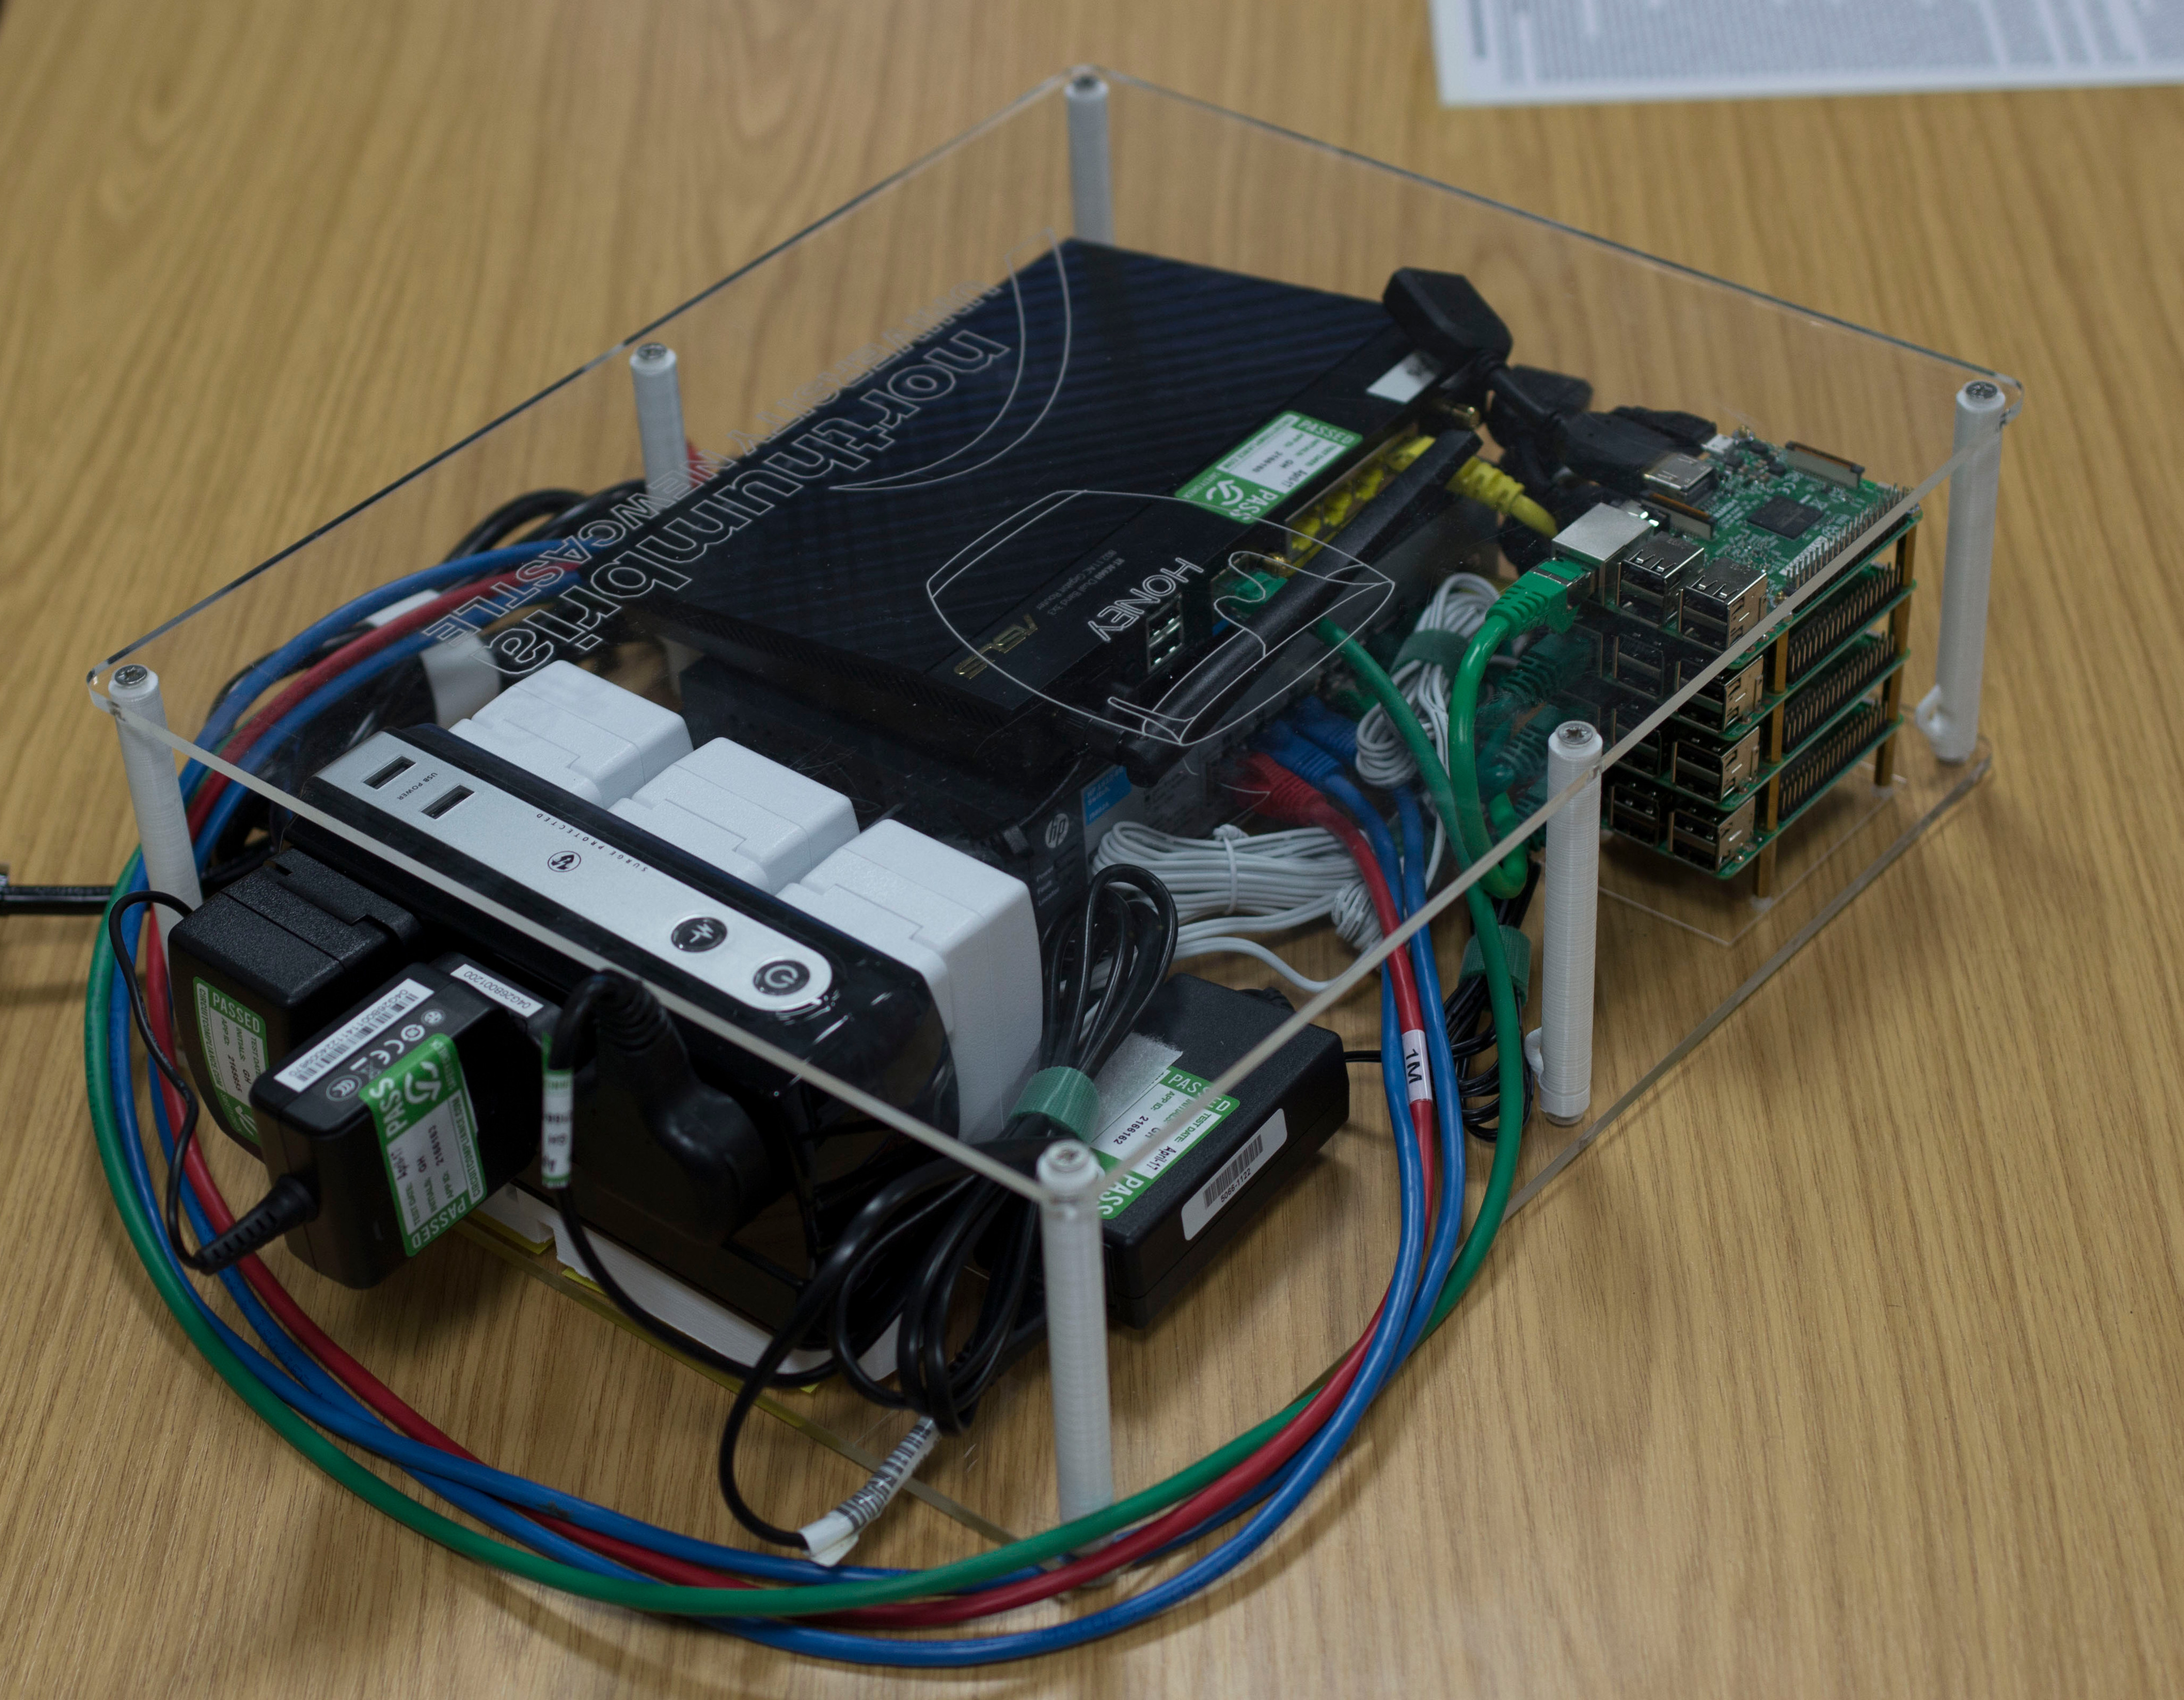
\includegraphics[width=\textwidth]{Images/HP1.eps}
%     \caption{\texttt{HILV} honeypot side view\label{fig:HP1}}
%   \end{minipage}
%   \hfill
%   \begin{minipage}[ht]{0.45\textwidth}
%     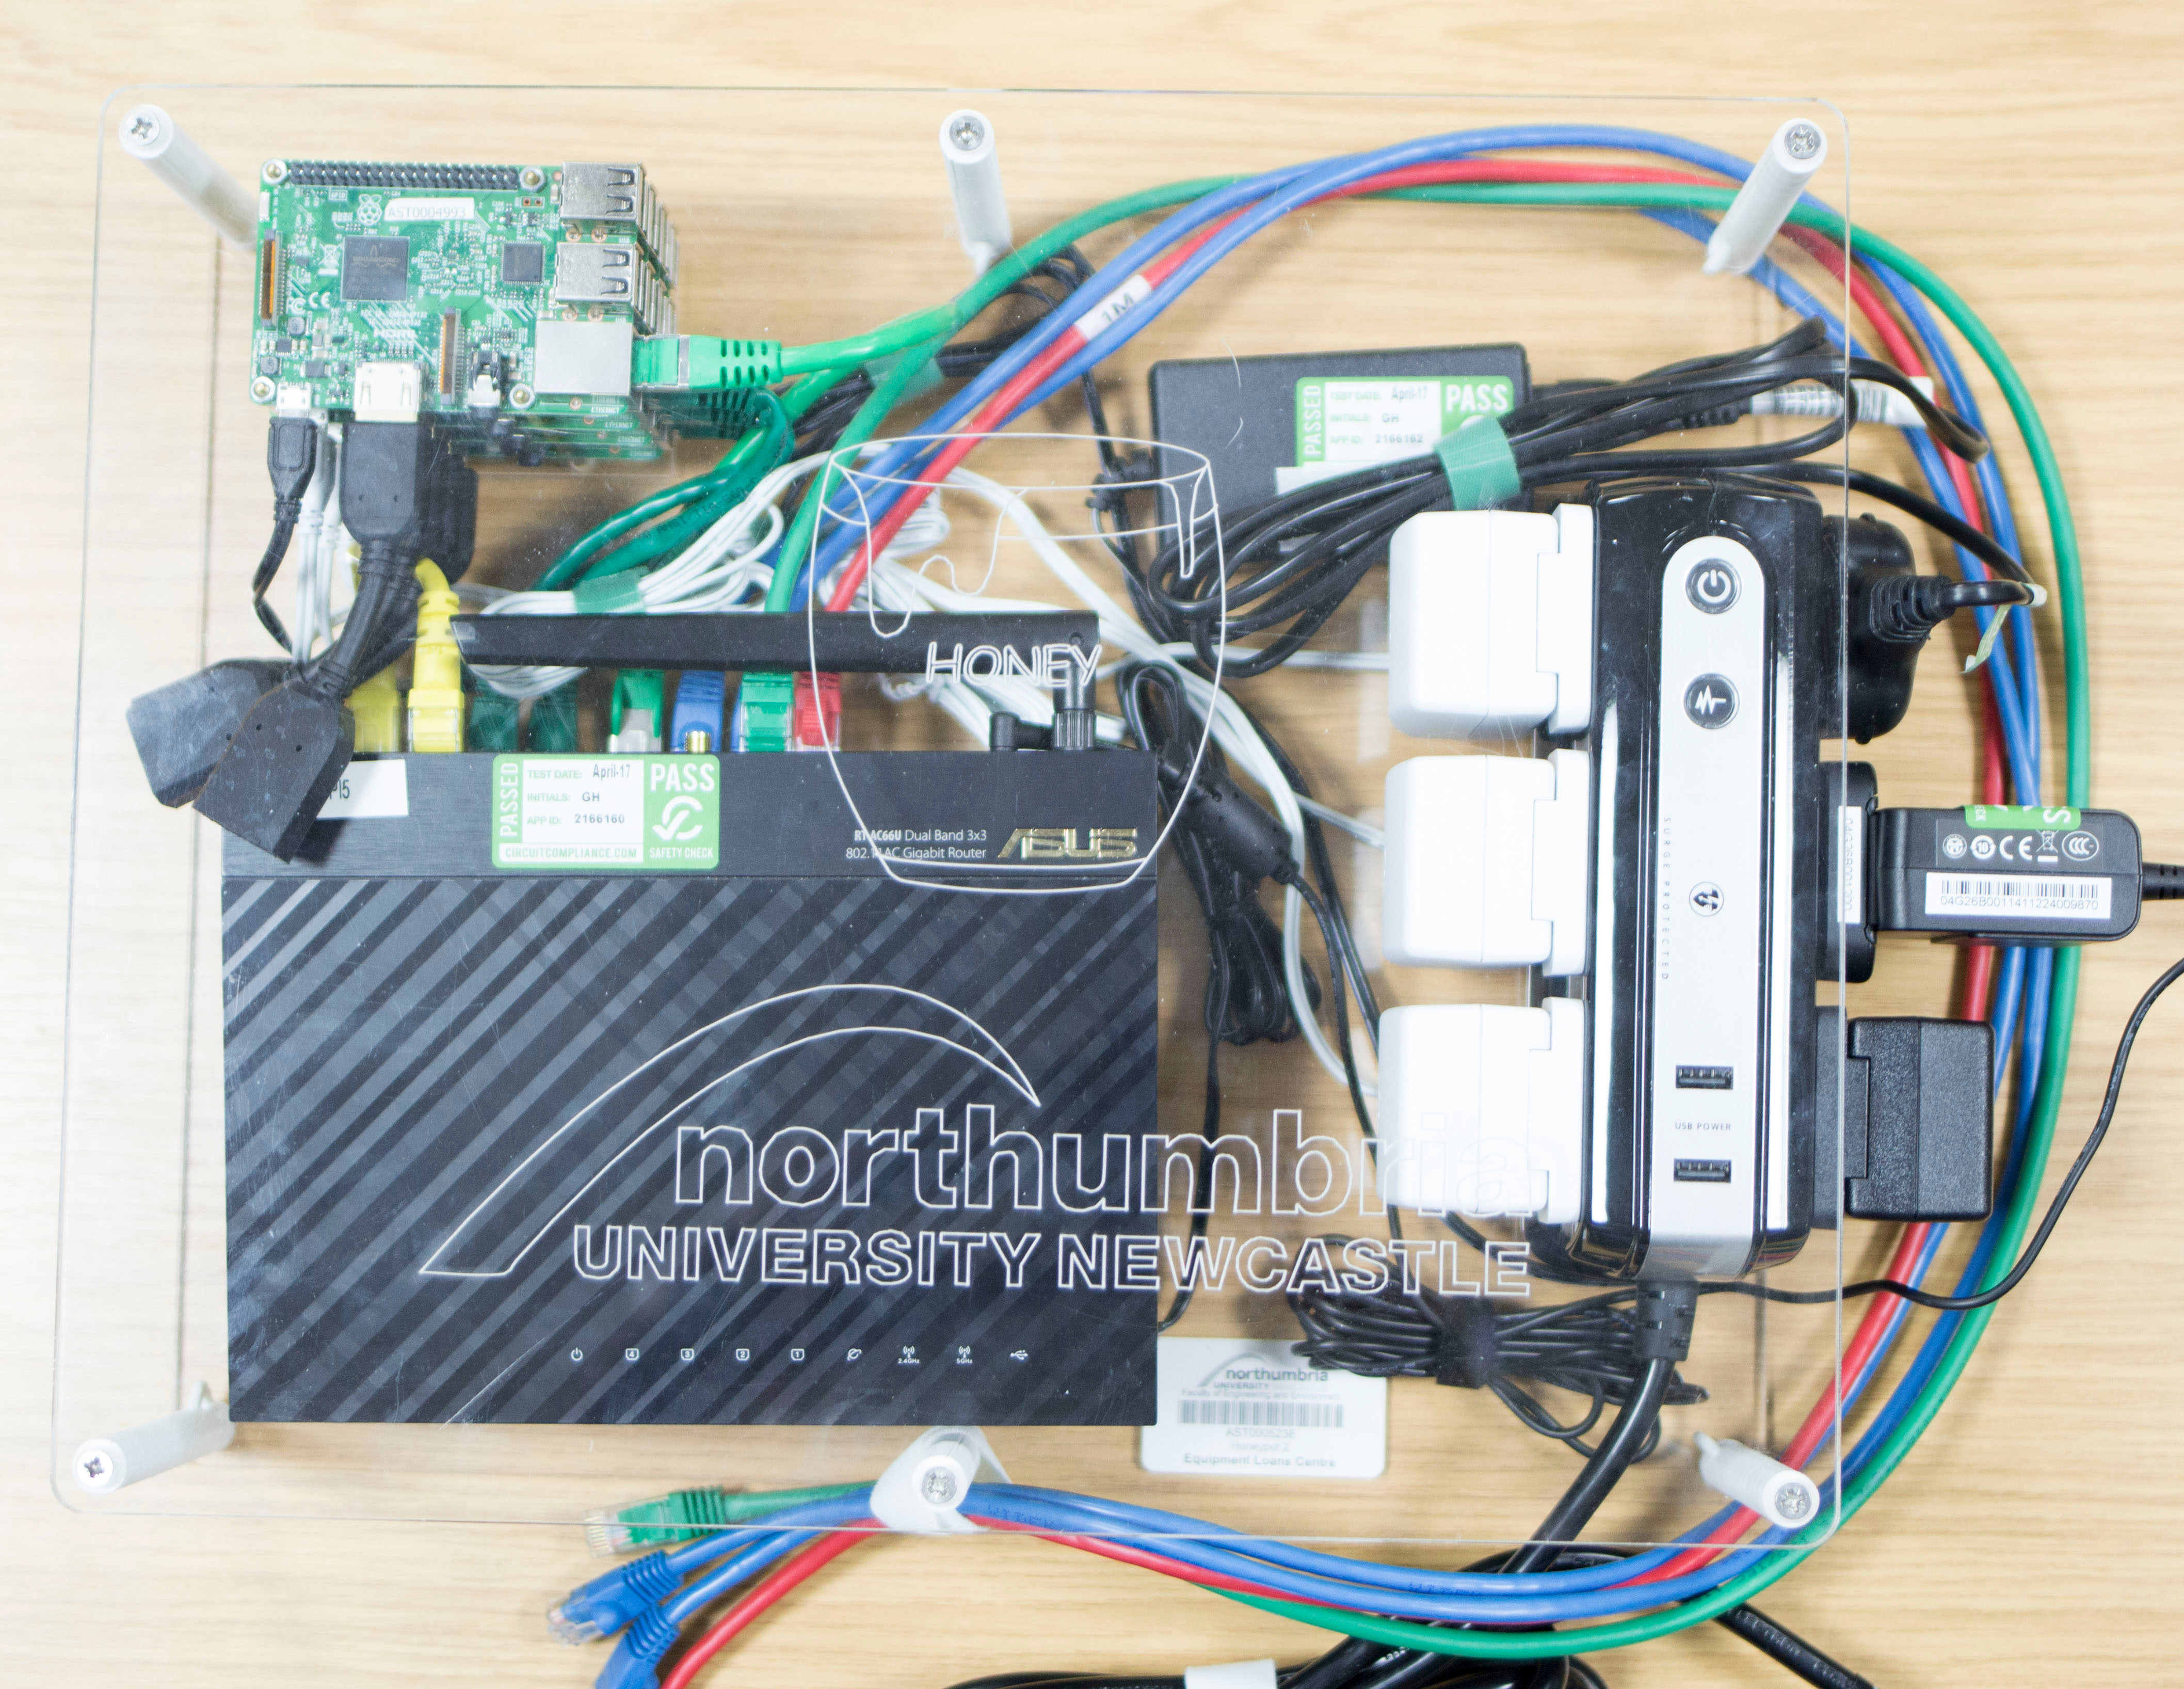
\includegraphics[width=\textwidth]{Images/HP2.eps}
%     \caption{\texttt{HILV} honeypot top view\label{fig:HP2}}
%   \end{minipage}
% \end{figure}

%% \begin{figure}[htb]
%% \begin{center}
%% 	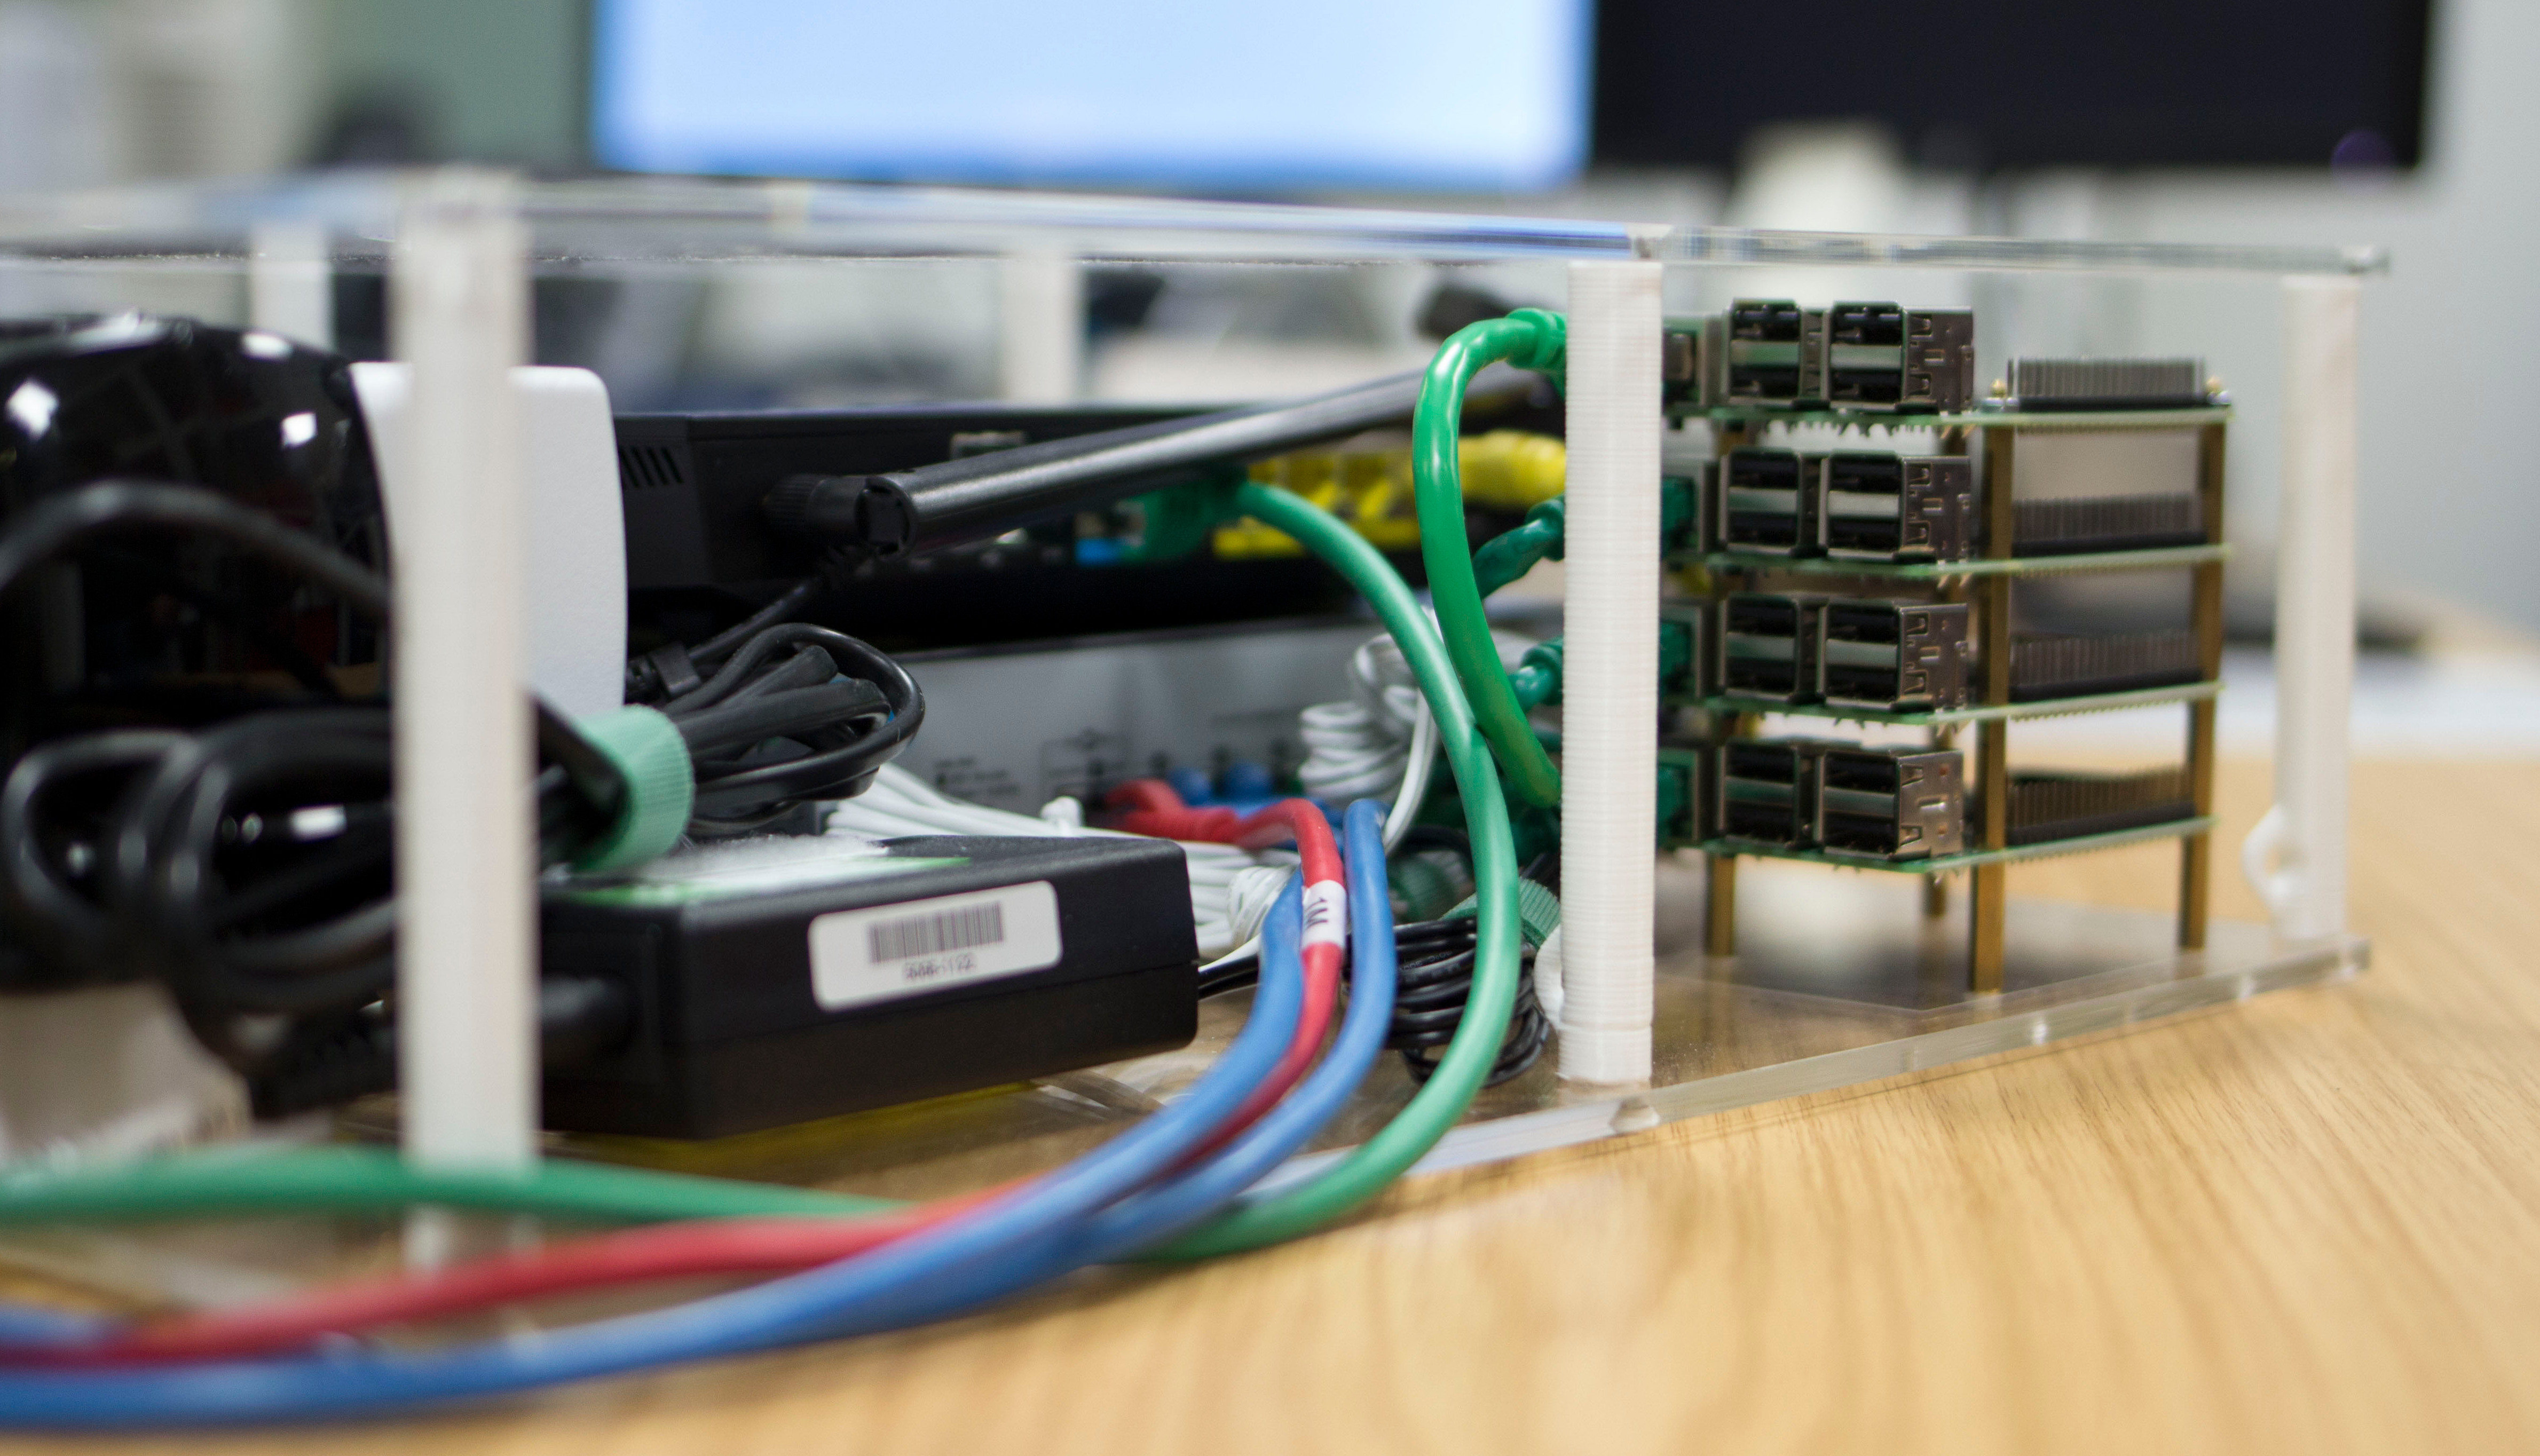
\includegraphics[scale=0.25]{Images/HP3.eps}
%% \caption{\texttt{HILV} Raspberry Pi boards (side view)}
%% \label{fig:HP3}
%% \end{center}
%% \end{figure}

The use of Raspberry Pi boards as the main servers for the honeypot simplifies
reconfiguration and rebuilding of the architecture.  The operating system (and
configured services) are stored on removable media (micro \texttt{SD} cards) which
simplifies server recovery and the maintenance of multiple configurations.
Images of the honeypot's base configuration can easily be restored. Multiple
configurations can be kept on different image sets and students can keep
individual projects as a set of micro \texttt{SD} cards that they retain for the
duration of a project.

The approximate cost of the basic \texttt{HILV} honeypot, without additional
devices or the monitoring PC attached, is $\approx$\pounds300 a breakdown of the costs is shown in Table~\ref{table:HILVCosts}. This offers a highly stimulating environment for the teaching of practical cybersecurity skills at a
very low cost.

\begin{table}[ht]
  \caption{\texttt{HILV} Costs\label{table:HILVCosts}}
  \begin{center}
  \setlength\doublerulesep{0.5pt}  
  \begin{tabular}{| l || c | c | c |}
  \hline
  \textbf{Product} & \textbf{Quantity} & \textbf{Unit Cost} & \textbf{Total} \\
  \hhline{|=||=|=|=|}
  \scriptsize{TP Link TL-SG108E 8 port switch} & \scriptsize{1} & \scriptsize{\pounds29.99} & \scriptsize{\pounds29.99} \\
  \hline
  \scriptsize{Raspberry Pi 3} & \scriptsize{4} & \scriptsize{\pounds33.00} & \scriptsize{\pounds132.00} \\
  \hline
  \scriptsize{Raspberry Pi PSU} & \scriptsize{4} & \scriptsize{\pounds8.89} & \scriptsize{\pounds35.56} \\
  \hline
  \scriptsize{TP Link TL-R470T+ Cable Router} & \scriptsize{1} & \scriptsize{\pounds34.99} & \scriptsize{\pounds34.99} \\
  \hline
  \scriptsize{Ethernet cables 1m (3 Pack)} & \scriptsize{1} & \scriptsize{\pounds15.31} & \scriptsize{\pounds15.31} \\
  \hline
  \scriptsize{Ethernet cables 0.25m (5 pack)} & \scriptsize{1} & \scriptsize{\pounds8.56} & \scriptsize{\pounds8.56} \\
  \hline
  \scriptsize{Masterplug 6 socket extension} & \scriptsize{1} & \scriptsize{\pounds16.99} & \scriptsize{\pounds16.99} \\
  \hline
  \scriptsize{Perspex Fabrication} & \scriptsize{1} & \scriptsize{\pounds30.00} & \scriptsize{\pounds30.00} \\
  \hhline{|=||=|=|=|}
   &  &  & \textbf{\pounds303.40} \\
  \hline
  \end{tabular}
  \end{center}
  \end{table}

\noindent\textit{\textbf{Address Range Support}}:
The \texttt{HILV} honeypot environment must reside on a different subnet from
the main laboratory network in order for the double \texttt{NAT}'d
configuration to function correctly. This is achieved by assigning a private
class~A \texttt{IP} address block, providing more than 16 million addresses.
\newline\newline

\noindent\textit{\textbf{Router Configuration}}:
The \texttt{HILV} honeypot's \texttt{ADSL} router is configured to provide only
routing services by disabling all other services, e.g.\ \texttt{NAS} and
\texttt{DHCP} facilities. This configuration allows all infrastructure
protocols to be managed from within the honeypot using small-scale servers
(Raspberry Pi boards). Configuring the services on separate
servers allows analysis of inter-service activity during normal network
activity and during an attack.

A low-cost router such as a \texttt{TP Link TL-R470T+}~\cite{TPLINKR470:18} is adequate for use in the \texttt{HILV} honeypot. The router is configured to use the laboratory-based \texttt{DHCP} server to acquire an  address. The \texttt{IP} address is
allocated from a reservation which allows a consistent mapping of the forwarded
\texttt{IP} address from the Internet-based router to the \texttt{HILV} honeypot
router. Defining the mapping in this way allows external host names
(\texttt{URL}s) to be mapped to the honeypot for Internet-based attack
analysis. Forwarding of traffic from the router into the honeypot
can be enabled and disabled when required.

For direct access to the honeypot from the laboratory, \texttt{IP} forwarding is
configured to  ``point'' to a target machine within the honeypot,
as shown in Fig.~\ref{fig:Forward}. In small-scale routers, this operation is
normally referred to as a \texttt{DMZ} (demilitarised zone) redirection~\cite{MB:01}.
\newline
\Figure[t!](topskip=0pt, botskip=0pt, midskip=0pt)[width=14cm]{Images/Forward}
{Address/Port forwarding\label{fig:Forward}}

% \begin{figure*}[ht]
% \begin{center}
% 	\includegraphics[scale=0.34]{Images/Forward.eps}
% \caption{Address/Port forwarding}
% \label{fig:Forward}
% \end{center}
% \end{figure*}

\noindent\textit{\textbf{Switch Configuration}}:

A key component of the \texttt{HILV} honeypot is a commercially available,
8-port, managed switch. The switch supports layer 2 management~\cite{ST:98} to
provide two specific technologies: port mirroring and port throttling. Suitable
switches include \texttt{HP 2530-08}~\cite{HP:17}, \texttt{TP-LINK
TL-SG2008}~\cite{TP:17}, and \texttt{TP Link TL-SG108E}~\cite{TPSG108E:18}.  The
combination of port mirroring and port throttling provides a reliable
architecture for packet capture.  \newline\newline

\noindent\emph{Port mirroring}:
Switches maintain an in-memory table of ports and \texttt{MAC} addresses to
support the efficient delivery of frames. This ensures that packets are transferred port to port rather than being broadcast. port to port communications are known as ``virtual circuits''. This
technology complicates the process of packet capture. When using a honeypot, packet
capture is a vital part of the architecture for the analysis of any
network-based attack vector. Using a managed switch (as discussed above), it is
possible to configure the ports on the switch to be mirrored to a specific
port, as shown in Figs.~\ref{fig:HPOverview} and~\ref{fig:throttling}. This
allows all the network activity to be captured and analysed~(\emph{Requirement
8}). Switches can implement mirroring in one of two ways. Firstly, a monitor-only
port can be provided, where the transmission capability of the port is removed,
(as in the case of an \texttt{HP 1810-G}). This type of configuration prevents the
monitoring device from adding traffic to the network. Alternatively, some
manufacturers configure the mirroring port to offer full transmit/receive
functionality, in addition to the mirroring capability (as in the case of a
\texttt{TP-SG108E}). This allows the attached monitor to also be used as a device within
the honeypot. If the monitor port provides full functionality, the addition of
a \texttt{LAN} tap~\cite{RB:13} can remove the transmission facilities of the port,
creating monitor-only functionality when required, as shown in
Fig.~\ref{fig:HPOverview}.
\newline\newline
\noindent\emph{Bandwidth throttling:}
A further issue with the capture of the honeypot network traffic is the
possibility of frame loss on the port to which the mirrored traffic is
forwarded.  Switches are designed to provide maximum transfer speed between
ports. This is achieved through the switch's backplane. If the throughput of
traffic on the mirrored ports exceeds the bandwidth of the port to which the
traffic is mirrored, then frame loss at this port is inevitable. To prevent
this occurring the switch must be configured to throttle the throughput on the
mirrored ports so as not to overwhelm the backplane.
Figure~\ref{fig:throttling} shows the basic configuration of a throttled
environment. The port which has the frames forwarded to it must be configured
to run at a speed that exceeds the total bandwidth of the mirrored ports. The
effect of this is that as frames are transferred between ports they are
reliably replicated via the backplane to the monitor port. This configuration
satisfies requirement 8.

\Figure[t!](topskip=0pt, botskip=0pt, midskip=0pt)[width=7cm]{Images/Throttle.eps}
{Port throttling\label{fig:throttling}}

% \begin{figure}[ht]
% \begin{center}
% 	\includegraphics[scale=0.4]{Images/Throttle.eps}
% \caption{Port throttling\label{fig:throttling}}
% \end{center}
% \end{figure}

\noindent\textit{\textbf{Internet Support}}:
Access to the Internet from the honeypot is possible through the double
\texttt{NAT}'d configuration. This configuration provides isolation from the
laboratory and the Internet. External response to a service request from a
device in the honeypot is achieved through packet forwarding, as shown in
Fig.~\ref{fig:Forward}. For this technique to function correctly the laboratory
network and honeypot network must be on different subnets.

The Internet facility also supports \texttt{IP} address forwarding to allow
Internet-based access into the honeypot. From the Internet, packets are
forwarded to the address of a honeypot router which, in turn, forwards traffic
to a target machine inside the honeypot, as shown in Fig.~\ref{fig:Forward}.

This configuration allows specific configurations to be exposed in order to
capture Internet-based attacks and to support remote access to the honeypot for
remote configuration and monitoring.

\subsection{\texttt{LIHV} Honeypot}

The \texttt{LIHV} honeypot is not intended for use in a reconfigurable
environment and does not require any monitoring or control of the network. No
port monitoring or throttling is required and all activity monitoring is
achieved using log files. The log files are made available 
for analysis of service-based access activity via a web-link.

The \texttt{LIHV} honeypot is a single 1U \texttt{LAMP} server (\texttt{HPE ProLiant DL360 Gen9 Server}~\cite{HPE:17} costing approx \pounds2000), located in a
separate cabinet, shown in Fig.~\ref{fig:Overview2}. The cabinet is secured to
prevent students having direct access to the hardware. It supports the general
honeypot service to provide students with a platform to carry out simple
authentication attacks using tools such as \texttt{Hydra} from within the
\texttt{Kali Linux}~\cite{OS:17} toolset. This honeypot also provides a target
for the development of bespoke authentication attack tools in the final year
undergraduate cybersecurity modules.  This server is accessed directly in the
laboratory or via the Internet as a bastion server~\cite{MB:05}. This allows
access from within the laboratory but also from outside the laboratory to
support directed learning tasks and also to support collaborative ventures.

\Figure[t!](topskip=0pt, botskip=0pt, midskip=0pt)[width=7cm]{Images/Infrastructure2.eps}
{\texttt{LIHV} honeypot overview\label{fig:Overview2}}

% \begin{figure}[ht]
% \begin{center}
% 	\includegraphics[size=14cm]{Images/Infrastructure2.eps}
%   \caption{\texttt{LIHV} honeypot overview}
% \label{fig:Overview2}
% \end{center}
% \end{figure}

\subsection{General Networking Laboratory}

The flexible laboratory environment needs to provide a re-configurable physical
networking layer. This is provided by a structured cabling architecture as
shown in~Fig.~\ref{fig:Overview1}. 

\Figure[t!](topskip=0pt, botskip=0pt, midskip=0pt)[width=14cm]{Images/Infrastructure.eps}
{General networking laboratory overview\label{fig:Overview1}}

% \begin{figure*}[ht]
%   \begin{center}
%     \includegraphics[scale=0.5]{Images/Infrastructure.eps}
%   \caption{General networking laboratory overview}
%   \label{fig:Overview1}
%   \end{center}
%   \end{figure*}  

Internet access is provided by cascading each cabinet's ``internet switch'' to the central communication cabinet's ``internet switch''. A logical view of the internet facilities are shown in Fig.~\ref{fig:NetworkLogical}.

\Figure[t!](topskip=0pt, botskip=0pt, midskip=0pt)[width=7cm]{Images/NetworkLogical.eps}
{Logical view of internet access\label{fig:NetworkLogical}}

% \begin{figure}[ht]
%   \centering
%   \begin{minipage}[ht]{0.45\textwidth}
%     \includegraphics[scale=0.2]{Images/NetworkLogical.eps}
%   \caption{Logical view of internet access}
%   \label{fig:NetworkLogical}
%   \end{minipage}
% \end{figure}

The communications cabinet is secured; students are not allowed access to it,
in order to prevent them from reconfiguring the base network and the network
services equipment. Figure~\ref{fig:CommsCabinet} shows the main infrastructure cabling within the communications cabinet.  The cabinet also contains the primary \texttt{DHCP} and
\texttt{DNS} servers, a 1U intranet server, a database server and a
\texttt{NAS} drive as shown in Fig.~\ref{fig:CommsCabinetServers}. It also includes a \texttt{VDSL} fibre link from the \texttt{ISP}. In the case of Northumbria University, the provider is BT
Business~\cite{BT:17}. A \texttt{Draytek Vigor 2850}~\cite{DC:17} router is used to
manage the \texttt{ISP} connection. 

\Figure[t!](topskip=0pt, botskip=0pt, midskip=0pt)[width=7.5cm]{Images/CommsCabinet.eps}
{Communications cabinet\label{fig:CommsCabinet}}

\Figure[t!](topskip=0pt, botskip=0pt, midskip=0pt)[width=7.5cm]{Images/CommsCabinetServers.eps}
{Communications cabinet servers\label{fig:CommsCabinetServers}}

% \begin{figure}[ht]
%   \centering
%   \begin{minipage}[ht]{0.45\textwidth}
%     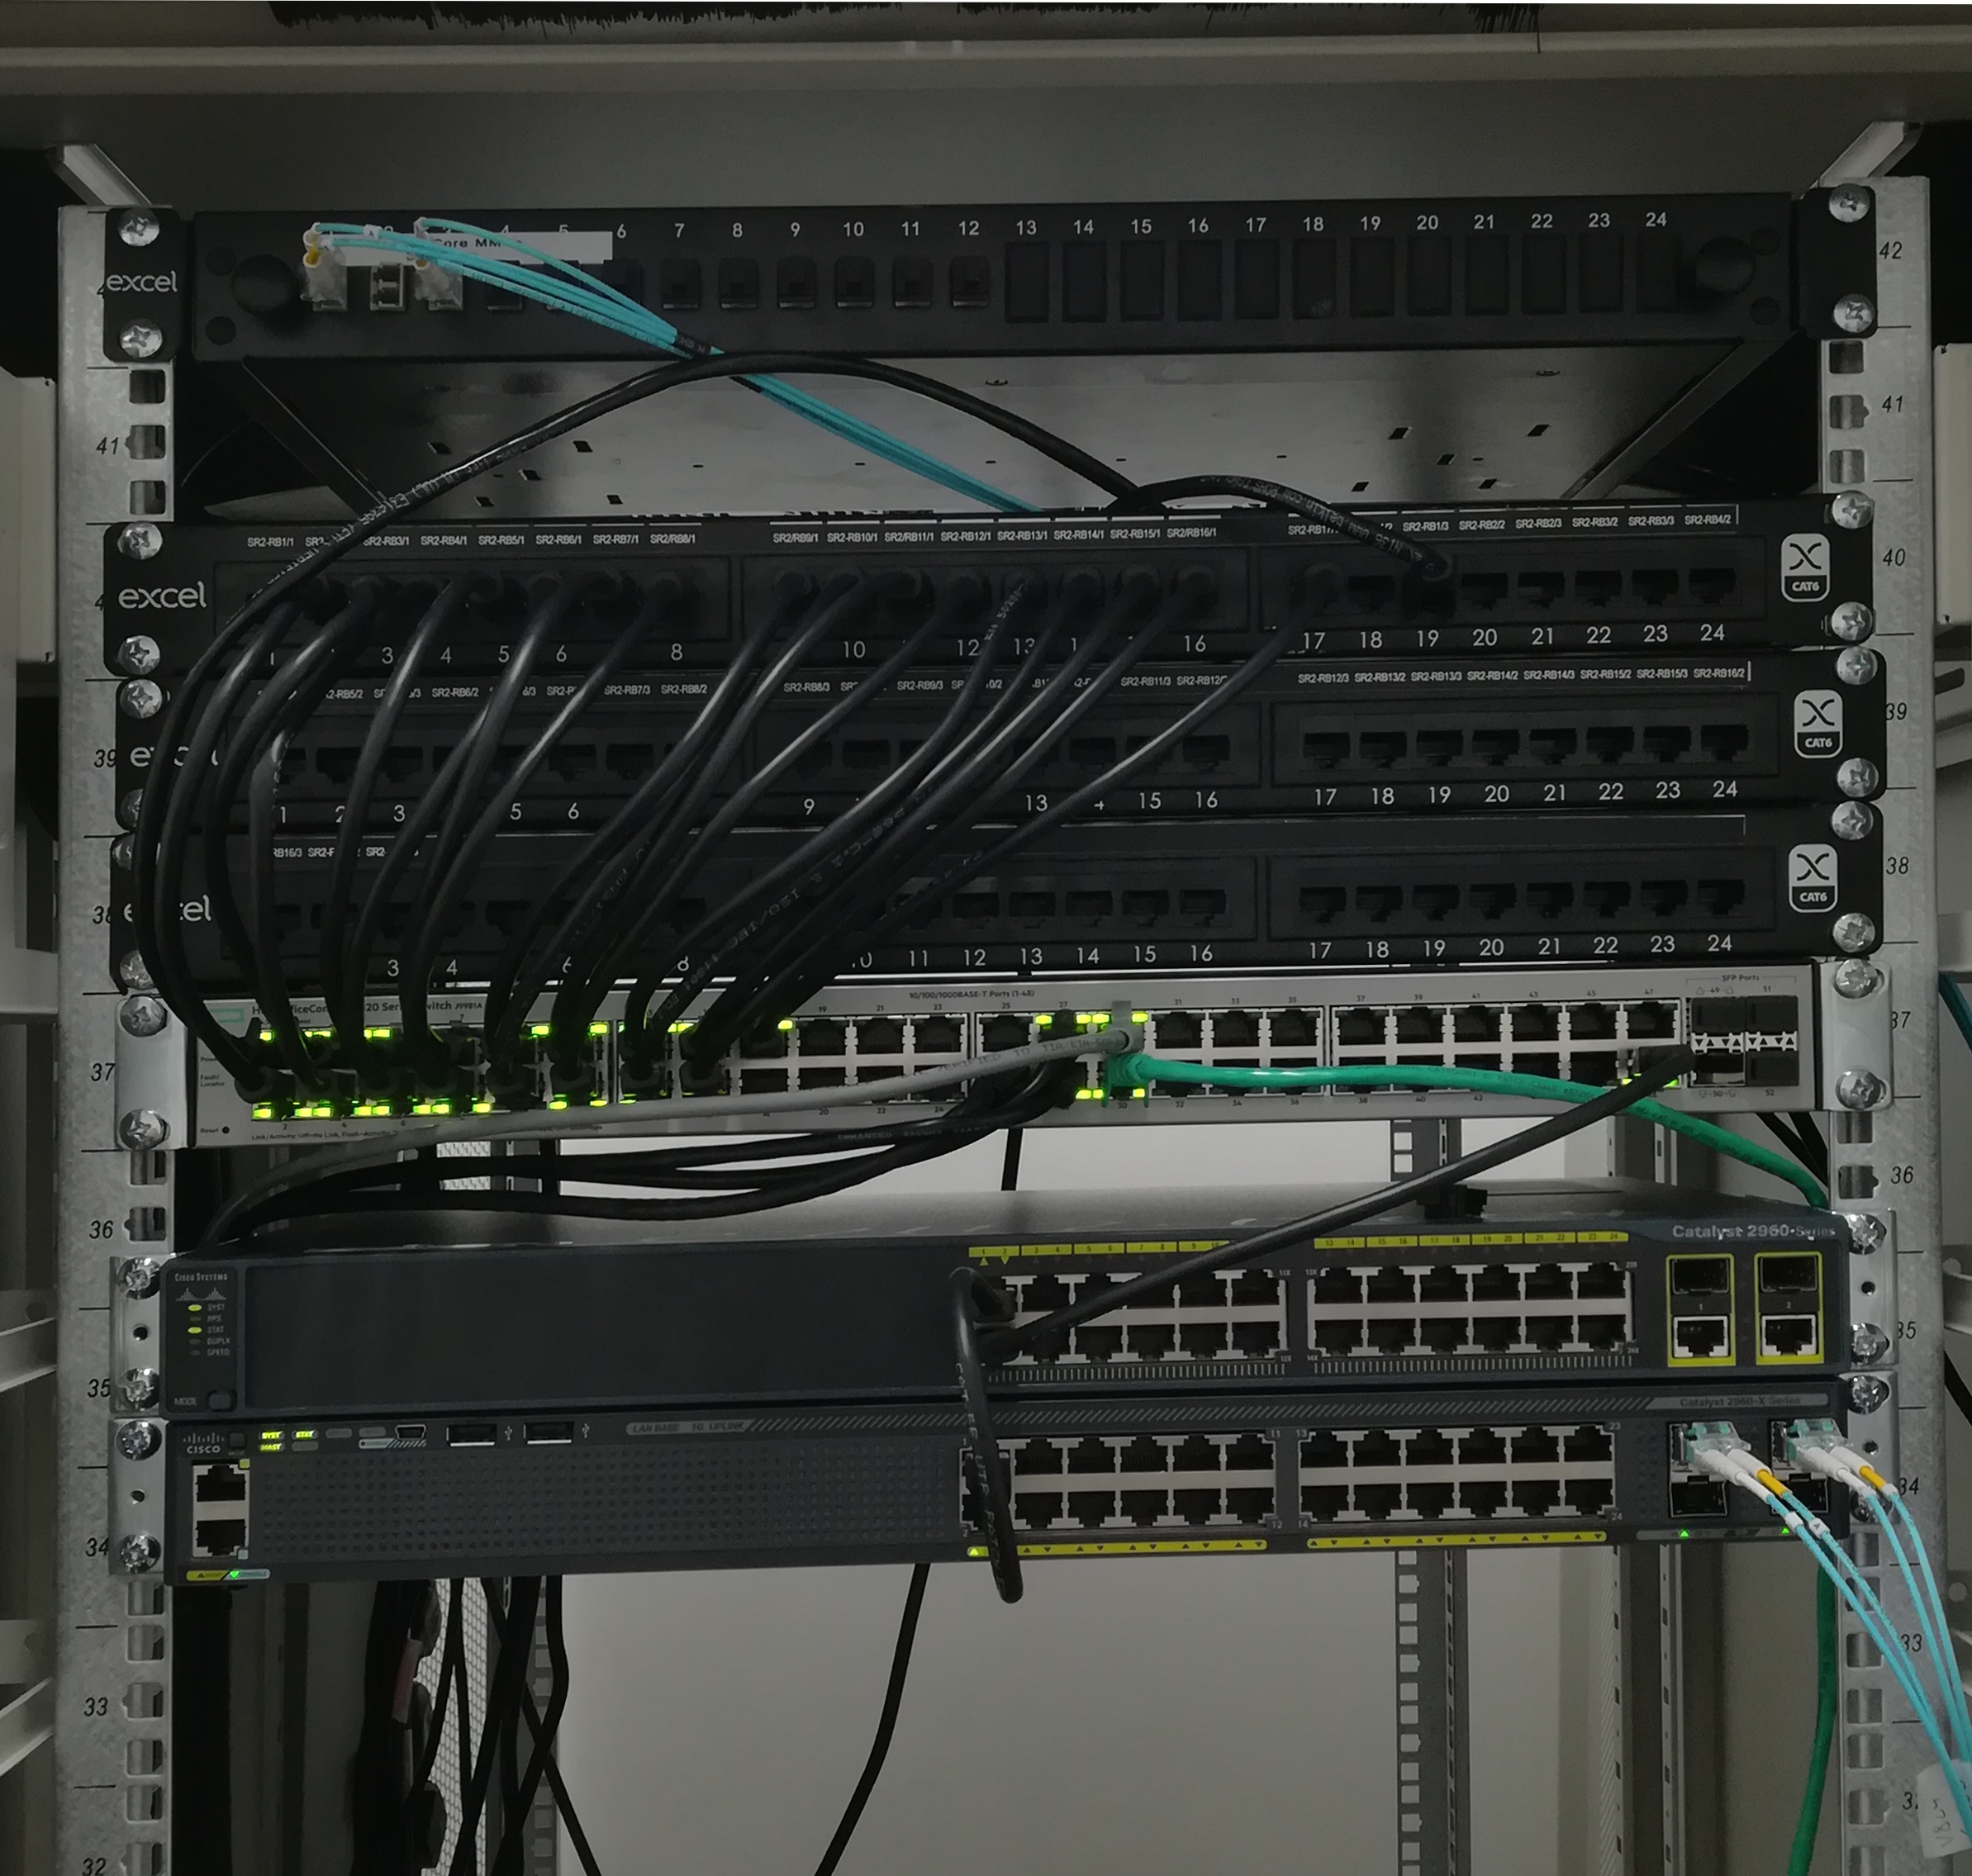
\includegraphics[width=\textwidth]{Images/CommsCabinet.eps}
%     \caption{Communications cabinet\label{fig:CommsCabinet}}
%   \end{minipage}
%   \newline
%   \begin{minipage}[ht]{0.45\textwidth}
%     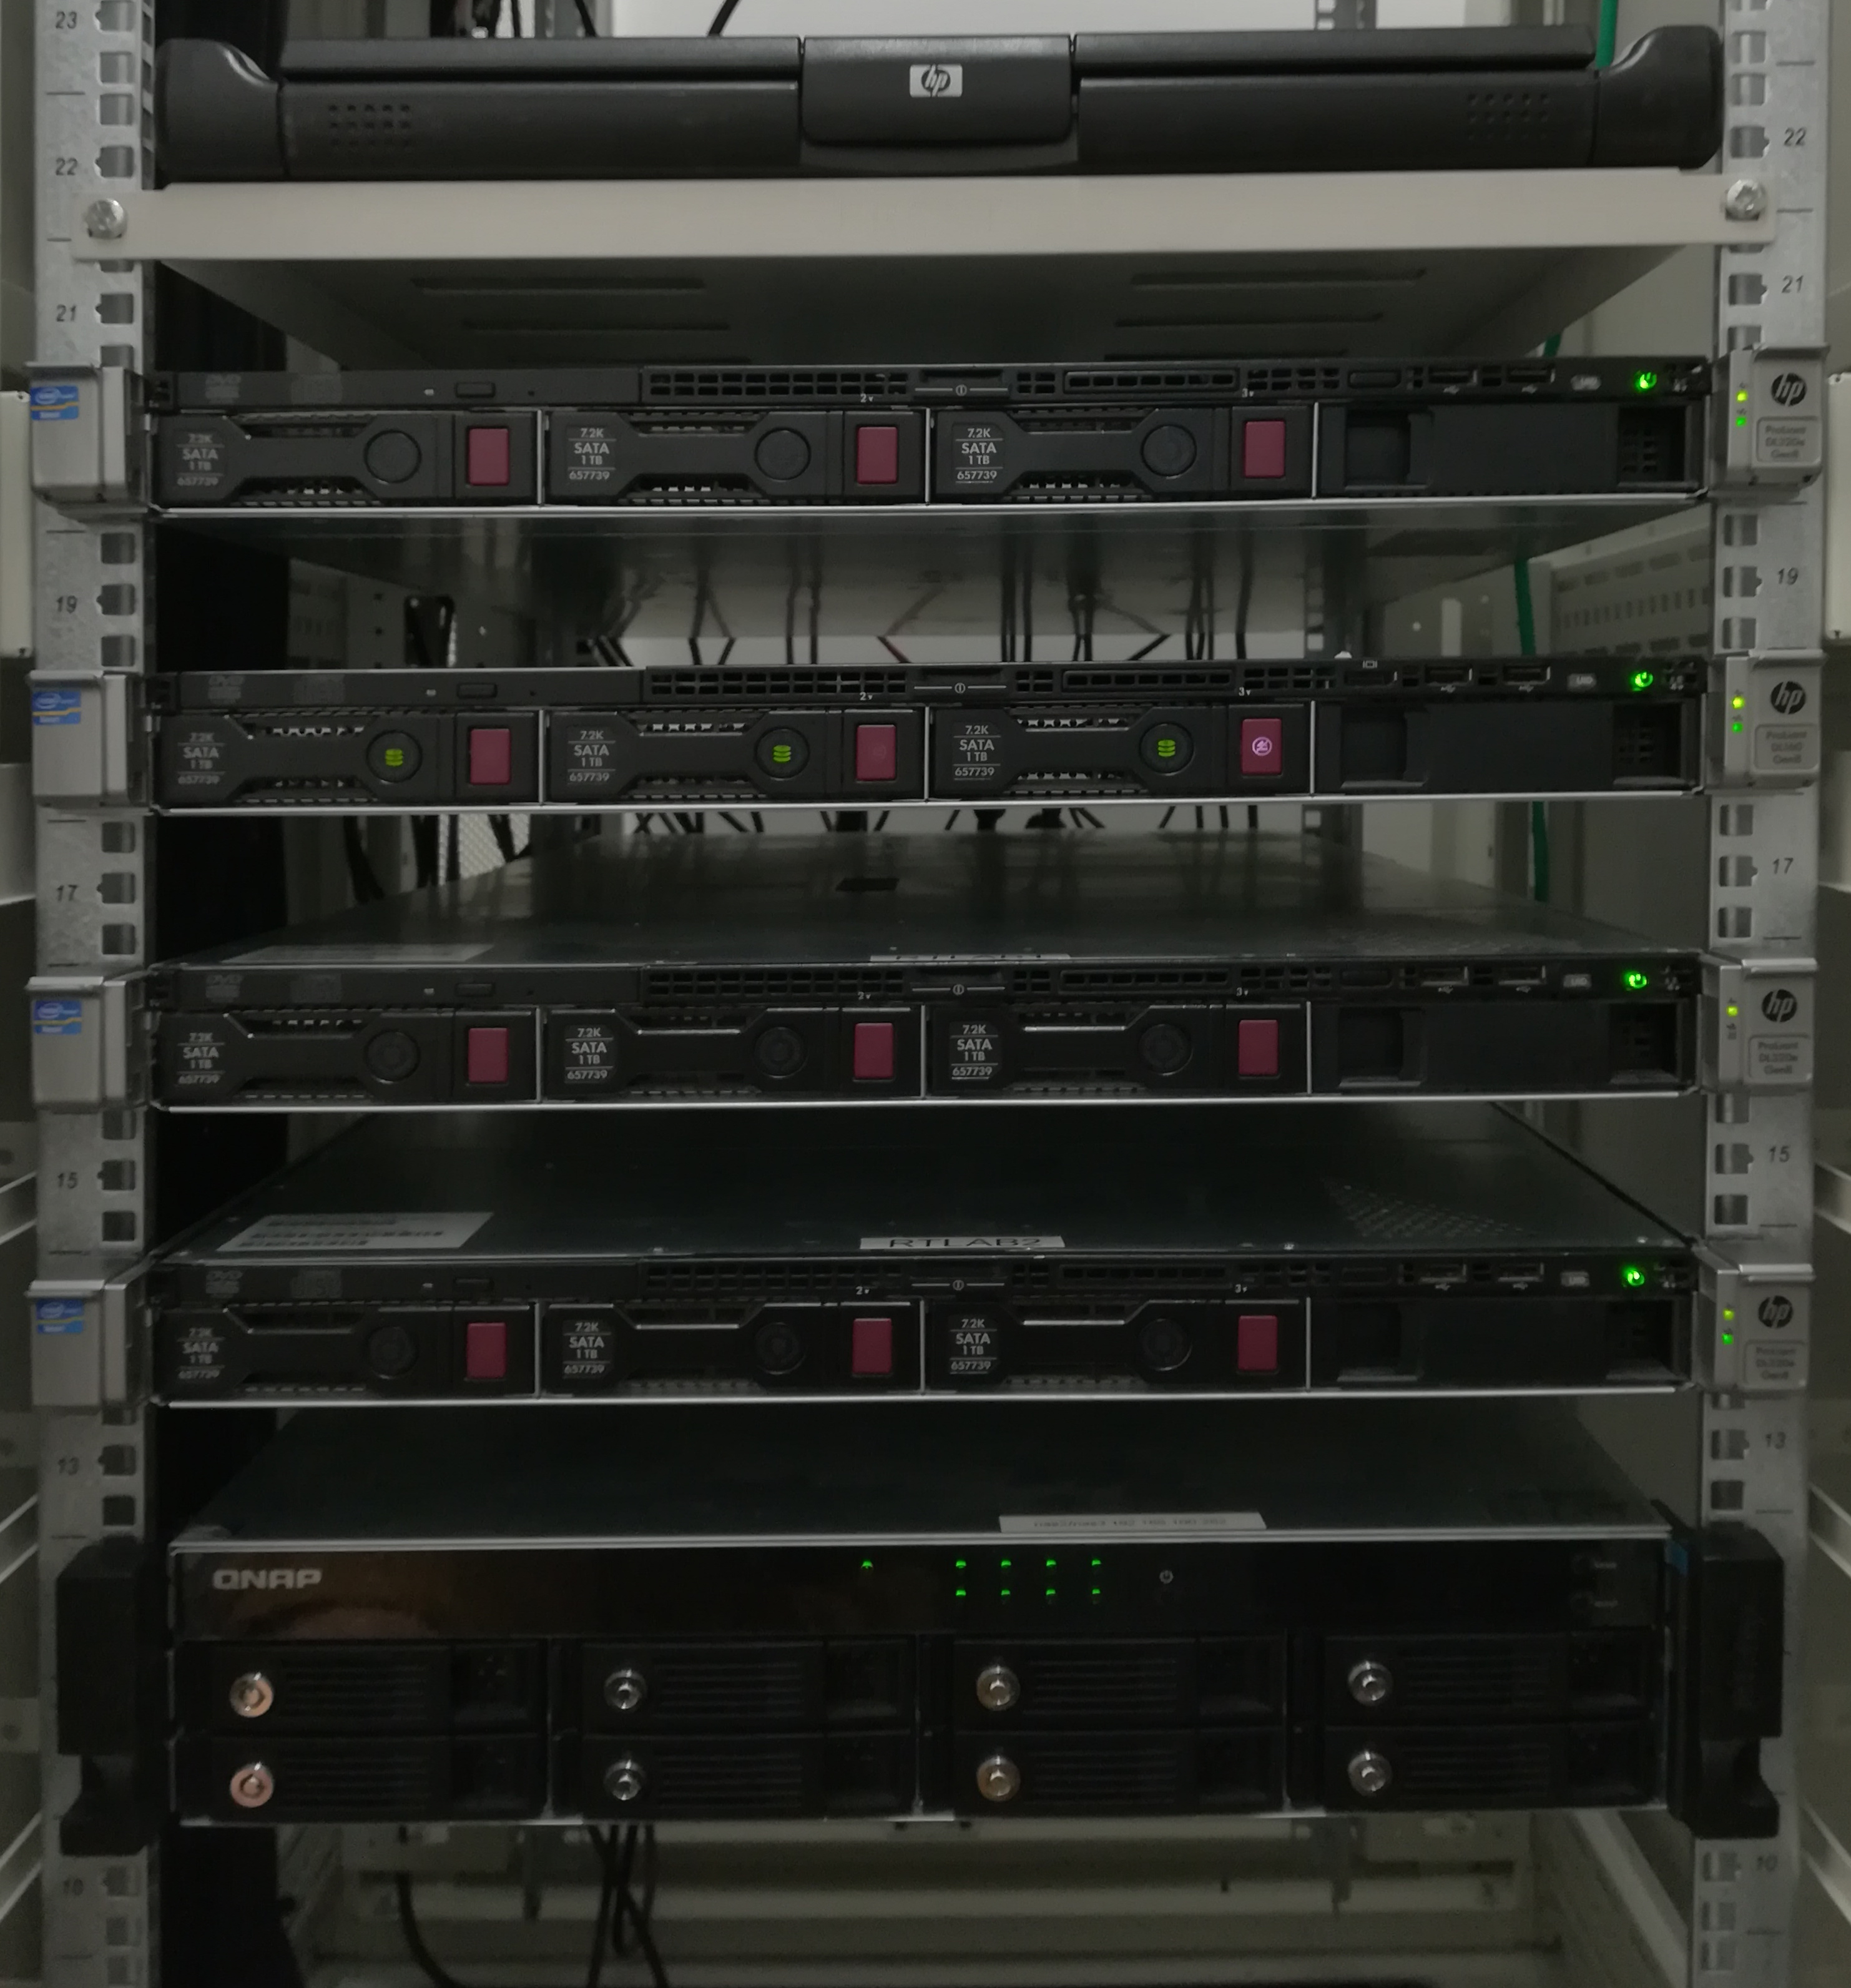
\includegraphics[width=\textwidth]{Images/CommsCabinetServers.eps}
%     \caption{Communications cabinet servers\label{fig:CommsCabinetServers}}
%   \end{minipage}
% \end{figure}

Students have unrestricted access to the other cabinets, each of which is
linked to a laboratory bench supporting 8--10 students, These cabinets contain a selection of switches, routers, \texttt{IP} Telephony, \texttt{IDS}, and Firewall equipment that is required for general network architecture modules as shown in Fig.~\ref{fig:Cabinet}.
They are linked back to the communications cabinet to provide internet access
for the benches. Access to the internet from the desktop is achieved through a
\texttt{NAT} connection from the \texttt{ISP} router in the communications
cabinet. 

\Figure[t!](topskip=0pt, botskip=0pt, midskip=0pt)[width=7.5cm]{Images/Cabinet.eps}
{General networking laboratory cabinet\label{fig:Cabinet}}

% \begin{figure}[ht]
%   \centering
%   \begin{minipage}[ht]{0.45\textwidth}
%     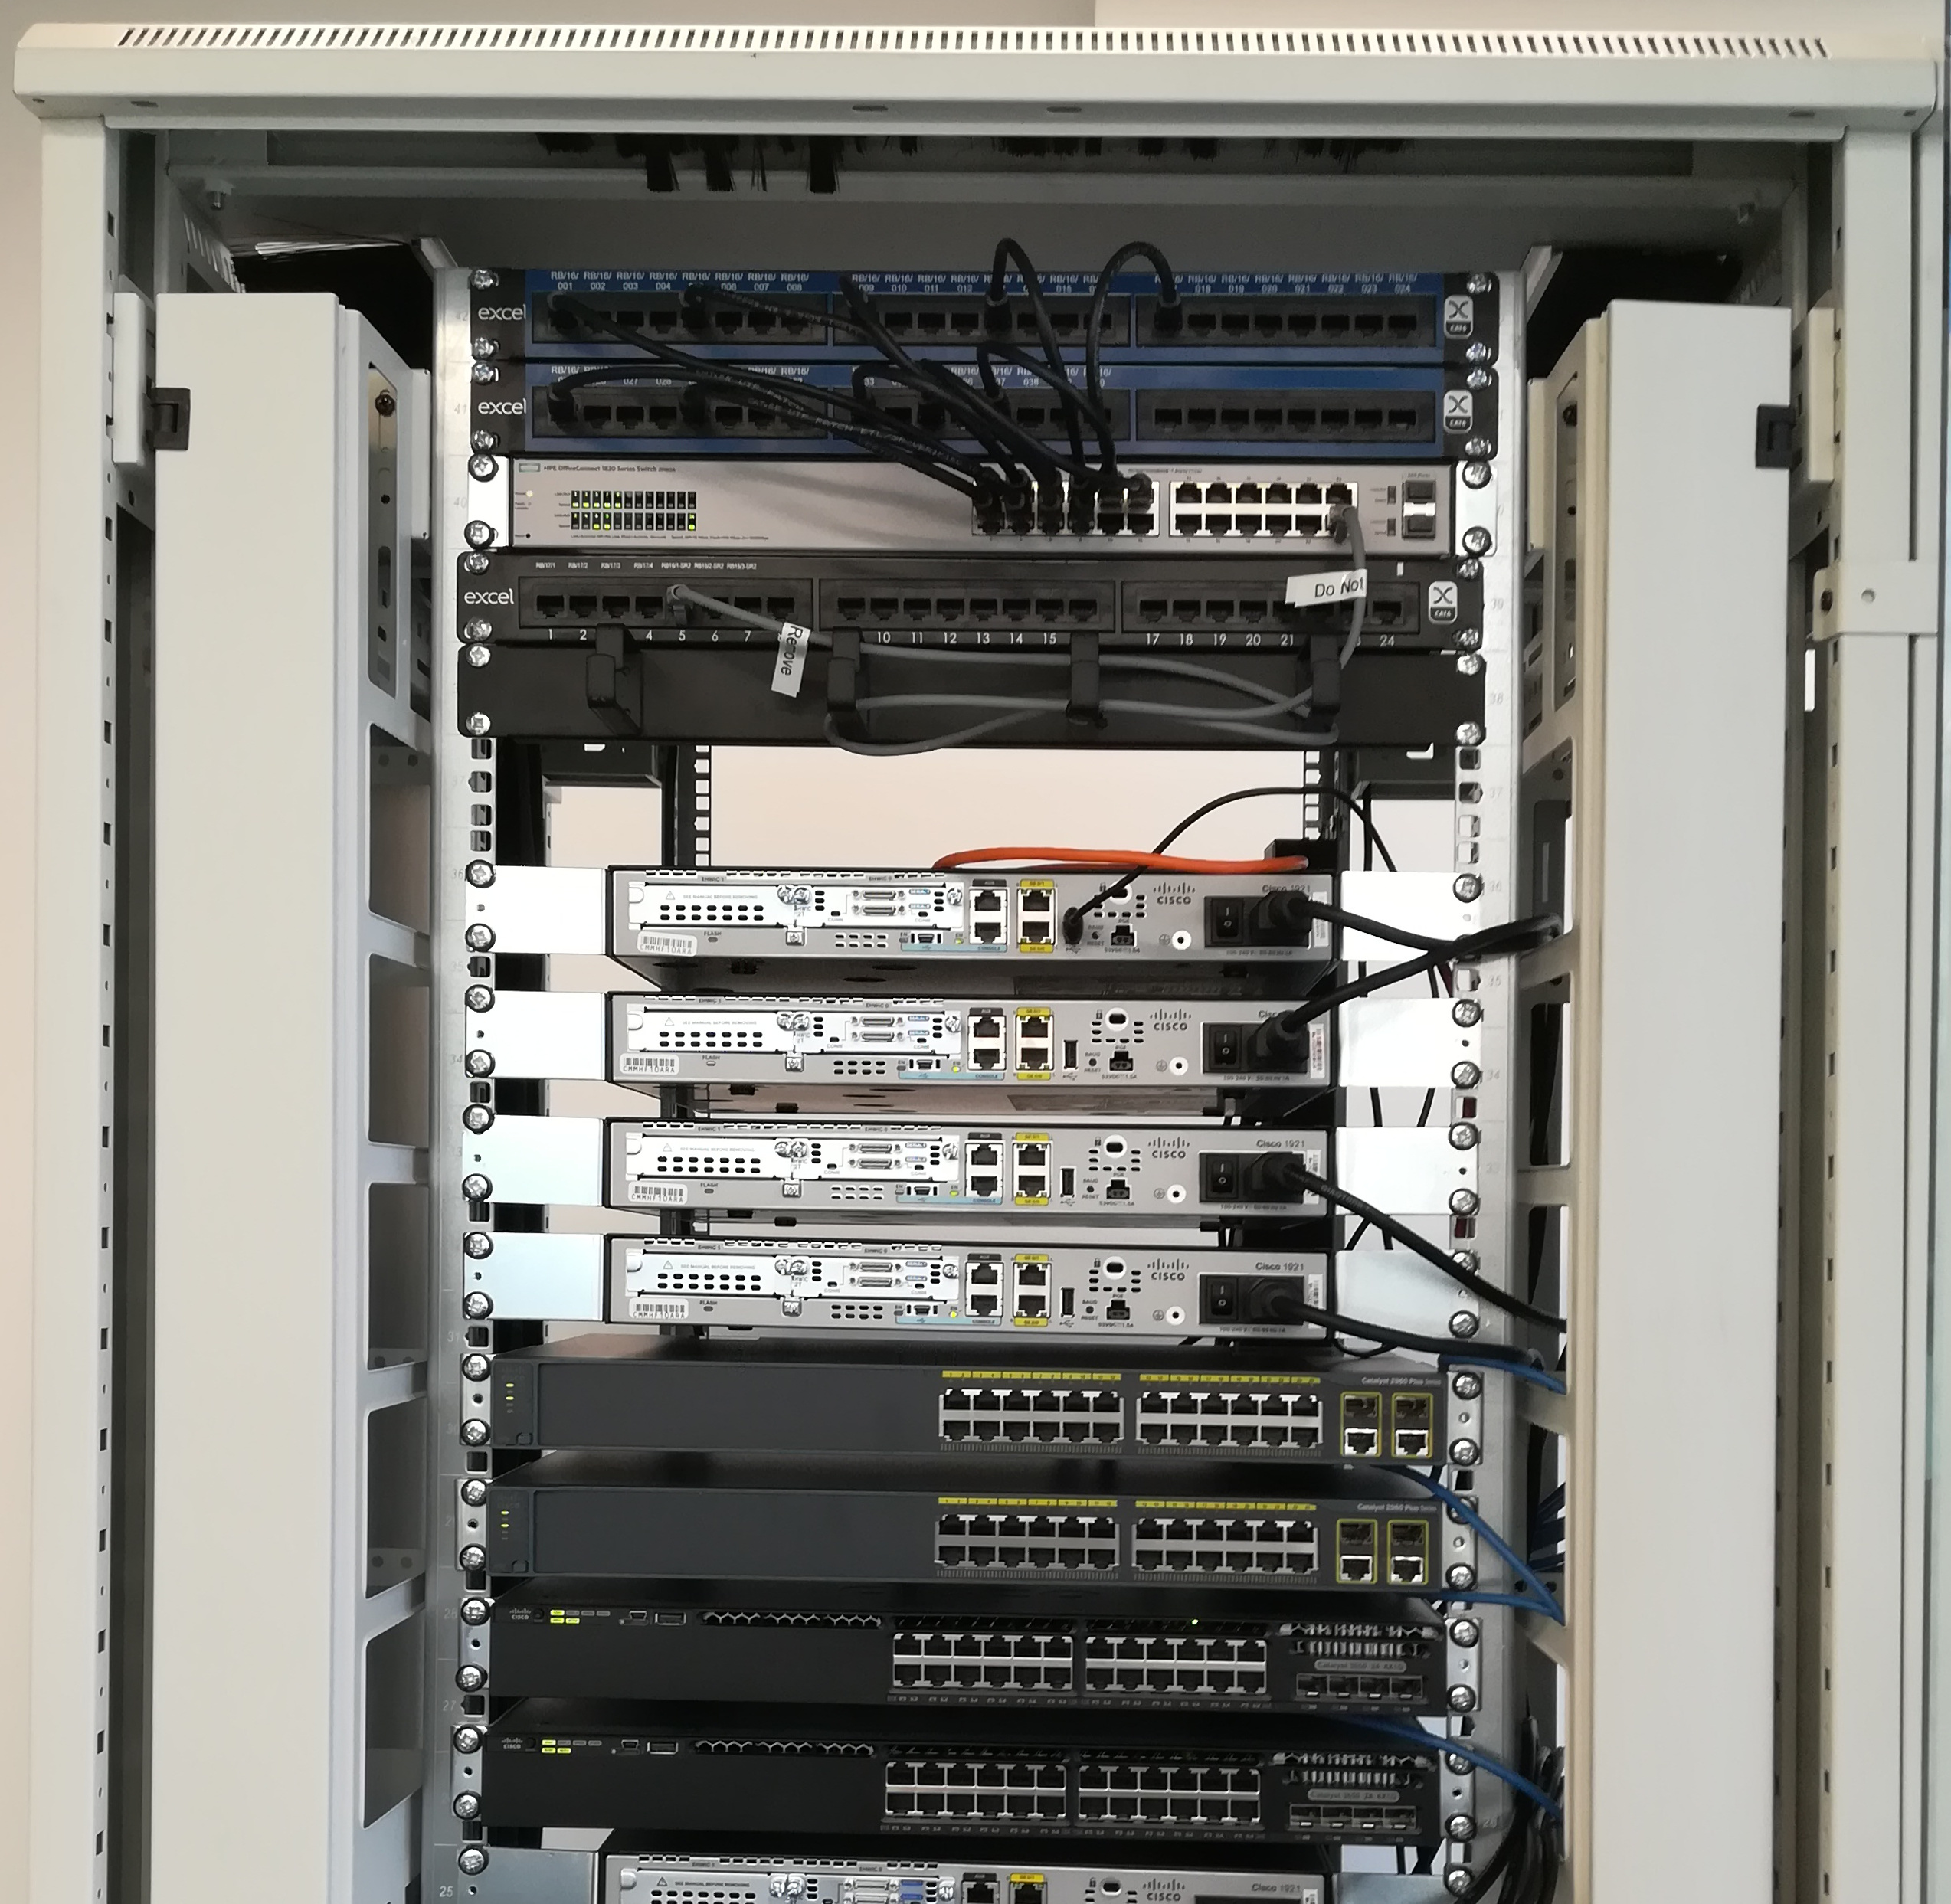
\includegraphics[width=\textwidth]{Images/Cabinet.eps}
%     \caption{General networking laboratory cabinet\label{fig:Cabinet}}
%   \end{minipage}
% \end{figure}

The structured cabling allows the resources of each cabinet within the
laboratory to be linked to the desktop through structured cabling ports.
Cross-cabinet connections ensure specialist resources are flexibly available to
all benches e.g.\ switches, routers, firewalls, and \texttt{IDS} (Intrusion
Detection Systems) etc.

\subsection{Address Range Support}

The use of virtualisation at the desktop (\texttt{GNS3}~\cite{GNS3:17},
\texttt{VMWare}~\cite{VMWARE:17} and \texttt{VirtualBox}~\cite{O:17}), to support operating
systems and networking modules, requires a large number of host addresses to
support a large number of students deploying statically addressed virtual
hosts. The base laboratory network infrastructure is configured as a single
class B subnet.  This provides 65,534 addresses, which is more than enough for
each student to be allocated a block of contiguous \texttt{IP} addresses for
each module, allowing multiple modules to be delivered concurrently without
having \texttt{IP} address conflicts.  This approach also allows equipment to
be moved around in the laboratory without requiring address reconfiguration.

\subsection{Network Service Deployment}\label{InfraService}

To support the study of operating systems and other general computing subjects,
the network requires, as a minimum, \texttt{DNS}~\cite{RA:11} and
\texttt{DHCP}~\cite{DL:02} services. These services are deployed across three
small-scale, 1U servers (\texttt{HPE ProLiant DL360 Gen9 Server}~\cite{HPE:17}). Two
servers are located in the communications cabinet as shown
in~Fig.~\ref{fig:Overview1}. One server supports \texttt{DHCP} and \texttt{DNS}
which are integrated to create a \texttt{DDNS}~\cite{SV:06} environment. The
second server acts as the secondary \texttt{DNS} server. The third server is
located in the \texttt{LIHV} honeypot cabinet and acts as a further secondary
\texttt{DNS} server.

The communications cabinet also contains a 1U server that provides the
laboratory intranet (\texttt{LAMP} based) service, along with general purpose
\texttt{MySQL} database services for the intranet and module content delivery.

Deployment of known desktop equipment is coordinated by creating reservation
entries in the \texttt{DHCP} service. The \texttt{DHCP} server then
automatically creates the forward and reverse \texttt{DNS} entries in the
\texttt{DNS} architecture as the equipment boots. Students can also connect
their own devices which are allocated a network configuration from a
\texttt{DHCP} address pool.

\subsection{Teaching Facilities Support}

Teaching of standard technologies, such as switching and routing, use the
physical equipment within the cabinets. The laboratory also supports network
virtualisation through \texttt{GNS3}, which can be integrated with the physical
equipment when necessary. The teaching of the \texttt{OS}-based technologies is
supported through the use of desktop virtualisation, allowing each student to
have multiple clients and servers running simultaneously on a single machine.
For large-scale scenarios, which are required on some modules, the virtual
machines may be deployed across several desktop machines. These large scale
deployments require the virtualisation software to support network card
bridging to allow the virtual machines to be ``physically'' connected to the
laboratory infrastructure.  Subjects that require a laboratory
``search-by-name'' facility (\texttt{DNS} and \texttt{rDNS}) such as Java
Sockets and C Sockets programming are supported by the \texttt{DDNS}
implementation as discussed in~Sect.~\ref{InfraService}.

\section{Operational Results and supported teaching}\label{sec:Results}

The general laboratory infrastructure has been in place, and actively used, for
10 years. The \texttt{LIHV} honeypot has been in place for 9 years. The
honeypot was developed to support a cybersecurity module on an undergraduate
networking programme and has been used successfully in the teaching of basic
attack vectors such as port analysis, banner grabbing and service interaction
(\texttt{FTP} and \texttt{HTTP}) for taught modules and projects.

The \texttt{HILV} honeypots were designed and built 6 years ago and have been
used since 2012 (5 years) on undergraduate networking programmes. They have been
deployed in activities such as service redirection attacks, amplification
attacks and man-in-the-middle scenarios.

The use of Raspberry Pi boards in the \texttt{HILV} honeypots has allowed
diverse subjects to be taught more easily due to their use of removable media
to store the operating system. The setup time for laboratories and teaching
sessions has been dramatically reduced compared to our previous approach of
using small clusters of PC's with removable drives, this is reflected in the
students response to the configuration of the \texttt{LIHV} as discussed in
section~\ref{sec:Feedback}.

There have been several hardware changes to the \texttt{HILV} honeypots over
this time but the basic architecture has remained unchanged. The latest change
involved an upgrade from Raspberry Pi 2 to Raspberry Pi 3. The cost of layer 2
switches and their availability has also improved and they are now more
affordable. As new honeypots are fabricated, \texttt{TP-LINK} switches are being used in
preference to the more expensive HP switches. The \texttt{TP-LINK} switches do not
provide a fully implemented monitor port; this requires the inclusion of a
network tap as shown in Fig.~\ref{fig:HPOverview}.

\subsection{Supported Teaching\label{ResourceSupport}}

The current implementation of the laboratory supports \textgreater200 students. This
includes undergraduates studying networking ($\approx$40) and cybersecurity
($\approx$150), and postgraduates studying networking ($\approx$20). Each of our
programmes is delivered in modules. A typical undergraduate programme runs
around 10 modules concurrently e.g.\ networking technology (years 1, 2, 3 \&
4 with MComp), security case projects (Year 2), Sockets programming (year 3).
Each module requires $\approx$3~hours contact per week and $\approx$3~hours of
directed learning, which may require laboratory time.  In addition, the
laboratory supports many undergraduate and postgraduate cybersecurity projects
($\approx$80), including cyber attack analysis and general cybersecurity research
such as biometric-based multi-factor authentication and \texttt{IoT} (Internet
of Things) security projects.

\subsection{Supported Modules\label{Modules}}

All network engineering modules, across both undergraduate and postgraduate
programmes, involving routing, switching, \texttt{VLAN} deployment,
\texttt{MPLS} networking and \texttt{IP} telephony are successfully taught
using the general networking laboratory infrastructure.

Network service deployment using server operating systems (Windows and Linux)
for both undergraduate and postgraduate programmes is taught successfully in
the environment using virtual machine technologies. The network service
deployments include load-balanced \texttt{HTTP}, network file system
deployments (\texttt{NFS} and \texttt{SMB}), replication based \texttt{MySQL}
services and large scale \texttt{DNS} deployments.

The \texttt{HILV} honeypot environment has allowed aspects of network-based
infrastructure, specifically broadcast-based network services, to be taught as
a practical implementation rather than only as a simulation, and has allowed
students to develop complete network infrastructures integrated to the
Internet.

Cybersecurity modules are predominantly taught using the \texttt{HILV}
honeypots, particularly when looking at attack vectors that require packet
spoofing or resource exhaustion through the volume of traffic generation.

The \texttt{HILV} honeypots have also allowed analysis of live attacks from the
Internet without impacting on the local laboratory network. Activities such as
port scanning are passed through directly to the \texttt{HILV} honeypot without
exposing the laboratory infrastructure. Implementing multiple \texttt{HILV}
honeypots has allowed profiles of subnet scanning and attacks to be analysed by
students, providing them with a rich environment for experimentation and
analysis.

\subsection{Supported Projects\label{Projects}}
The \texttt{HILV} honeypots have been available for several years now and
students who move to the final year of the cybersecurity undergraduate
programme tend to carry out research-based projects. Usually these involve the
use of the basic \texttt{HILV} honeypot, but some projects add additional
components to the honeypot such as firewalls (pfSense~\cite{PFSENSE:18} or
ipFire~\cite{IPFIRE:18}) or wireless access points for the analysis of phone or
tablet based application attacks. A sample of recent projects is described below.

\begin{itemize} 
  \item \noindent \emph{Multi-Tiered defence analysis of a simulated cyber
    attack.} This project involved configuring the \texttt{HILV} honeypots to
    support a \texttt{IPFire} (software based firewall technology) and
    investigating potential tunnelling techniques that could compromise a
    military grade network deployment.  
  \item \noindent \emph{Development of a small \texttt{IDS}.} This project
    involved developing a \texttt{libpcap-}based application to run on one of the
    Raspberry Pi boards. The application monitored network
    traffic to identify a \texttt{SYN} flood attack using a simple window-based
    statistical analysis.  
    \item \noindent \emph{Attack on a secure \texttt{IoT} protocol} This
      project involved developing a network of \texttt{IoT} devices for
      environment analysis (temperature and humidity) and identifying the
      encrypted payloads within the traffic (\texttt{MQTT}) which was then attacked using a block
      decryption technique.  
    \item \noindent \emph{Development of an \texttt{IDS} for a full subnet
      \texttt{MitM} attack} This project involved developing a stateful 
      \texttt{IDS} using \texttt{libpcap} to identify spoofed \texttt{ARP} packets.  
    \item \noindent \emph{Development of a \texttt{DOS} tool that attempts to
      prevent detection from an \texttt{IDS}} This project involved developing
      a \texttt{RAW} sockets application that crafted packets to
      replicate valid traffic within the subnet environment.  
     \item \noindent \emph{Analysis of a \texttt{DNS} amplification attack} This
       project involved configuring a vulnerable \texttt{DNS} environment and
       executing an attack and analysing the bandwidth effect of the network.
\end{itemize}

\subsection{Student Feedback}\label{sec:Feedback}

In academic year 2017/18, following the delivery of the security case project,
we carried out a small survey to gauge student opinion about the effectiveness
of the laboratory configurations. We canvassed a cohort of 48 students of whom
30 responded. The results of the survey are summarised briefly below.
\begin{itemize}
  \item \noindent\emph{Utility:} Students were asked how useful they found the
\texttt{HILV} honeypot for the practical research component of the module. All
students found the honeypot useful, with 86.6\% rating the usefulness as very
useful or excellent. This result matched our expectations, as students usually
report that they learn better when they have access to physical equipment.
  \item \noindent\emph{Ease of use:} Students were asked how easy it was to
configure the \texttt{HILV} honeypot. This question related to scenarios in
which students were provided with a basic configuration and were required to
extend and adapt it to their own requirements. 98\% of students reported that
it was not difficult to configure the honeypot, with the majority indicating
that they found it easy or very easy.
\par\noindent This ease of use can be attributed to the following factors.
  \begin{itemize} 
    \item The base configuration of the honeypot has a fixed configuration for
      the router and switch, which allows students to sign out any of the
      honeypots from the loans facility and use it immediately in a
      `plug-and-play' fashion for many exercises.  
    \item The students created their own base servers from a set of images
      distributed from the laboratory \texttt{NAS} drive.  Following each
      practical session the students retained the \texttt{SD} cards for use at
      the next session. The \texttt{SD} cards provided a stateful configuration
      of their work.  
    \item The students were able to backup their entire project using a ``dump''
      (\texttt{dd}) of the \texttt{SD} cards.
  \end{itemize}
  \item \noindent\emph{Previous experience and likely future use}: Students
were asked if they had used a honeypot earlier in their studies. Most students
(93.3\%) had not used a honeypot before their undergraduate studies and
therefore had no preconception of what to expect. In contrast, when asked if
they would consider using the \texttt{HILV} honeypot again, the majority
(96.6\%) of the students indicated that they would use it for further studies. 
\end{itemize}
More extensive and more careful studies are needed to quantify the 
pedagogical benefits of our approach but these preliminary results are an 
indication of a very positive student reaction to their experience in our
laboratory.
\section{Conclusion and Future Work}\label{sec:ConclusionFuture}

The development of the \texttt{HILV} honeypot environment and its integration with the general purpose networks lab and the \texttt{LIHV} laboratory based honeypot has proved successful
for both teaching and research. The cost of the \texttt{HILV} honeypot deployment has been reduced
to such an extent that rather than the laboratory supporting the single \texttt{LIHV} honeypot
platform, which has to be reconfigured between sessions, the laboratory can now
support multiple honeypot deployments that are highly configurable and
portable.

As the \texttt{HILV} honeypots are small scale and low cost, the equipment is
permanently configured for teaching purposes. Each \texttt{HILV} honeypot is
capable of supporting four students at a time to work on research-based modules
and allows practical cybersecurity modules to be delivered more effectively.

The integration of the honeypots into a laboratory environment that supports
a wide-range of other technology-focused modules provides a cost-effective
solution to the delivery of stimulating, practical cybersecurity teaching.

Student numbers have risen sharply for cybersecurity courses and the
use of the honeypots has allowed additional levels of cybersecurity to be
incorporated into existing network courses. This has had a strategic impact on
the University since the B.C.S. (British Computing Society) added
cybersecurity as a required part of its accreditation process.

Our aim is to increase the number of \texttt{HILV} honeypots to accommodate the
increasing number of students. The low cost of the platform makes this an
achievable goal. It is also envisaged that, using this technology, the
department will be able to expand its cybersecurity research by preparing
students for PhD studies in the subject area. It is intended to seek funding to
develop a \texttt{HIHV} honeypot to support these PhD students. This honeypot
will consist of several large scale servers along with commercial grade
switches and routers and large-scale data capture facilities. Such a facility
will provide an excellent environment for the study of cybersecurity at PhD
level and has the potential to advance our understanding of the subject
significantly.

\bibliographystyle{IEEEtran}
\bibliography{honeypot}

\begin{IEEEbiography}[{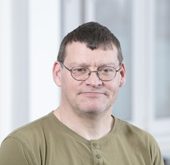
\includegraphics[width=1in,height=1.25in,clip,keepaspectratio]{Images/NE}}]{Neil Eliot}
is a Senior Lecturer at Northumbria University.  Neil was awarded his Ph.D. from Northumbria in 2017, his Pg.C. in 1994, and his B.Sc. in 1989 all in Computing. His research areas include swarm theory and cybersecurity. Neil is a Certified Ethical Hacker (CEH) and coordinator for the EC Council Academic alliance at Northumbria. He is also responsible for the delivery of several network cybersecurity modules in the area of operating systems integration, smart home technologies and modules that focus on cybersecurity threats in large scale system deployments. Prior to this Neil worked in the chemical industry and the NHS.
\end{IEEEbiography}

\begin{IEEEbiography}[{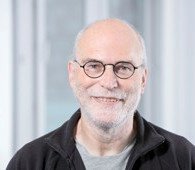
\includegraphics[width=1in,height=1.25in,clip,keepaspectratio]{Images/DK}}]{David Kendall}
has been a Senior Lecturer in Computing at Northumbria University since 1989, except for a brief period as a Lecturer in Computer Science at Durham University (2001-02). Previously, he was a Research Associate at Newcastle University (1987-89), following experience as a Senior Software Engineer in industry (1983-86). He has an M.A. degree in Literae Humaniores from Oxford University, where he studied at New College. He received M.Sc. and Ph.D. degrees in Computing Science from Newcastle University. His research interests are in the area of formal modelling and analysis of embedded systems. 
\end{IEEEbiography}

\begin{IEEEbiography}[{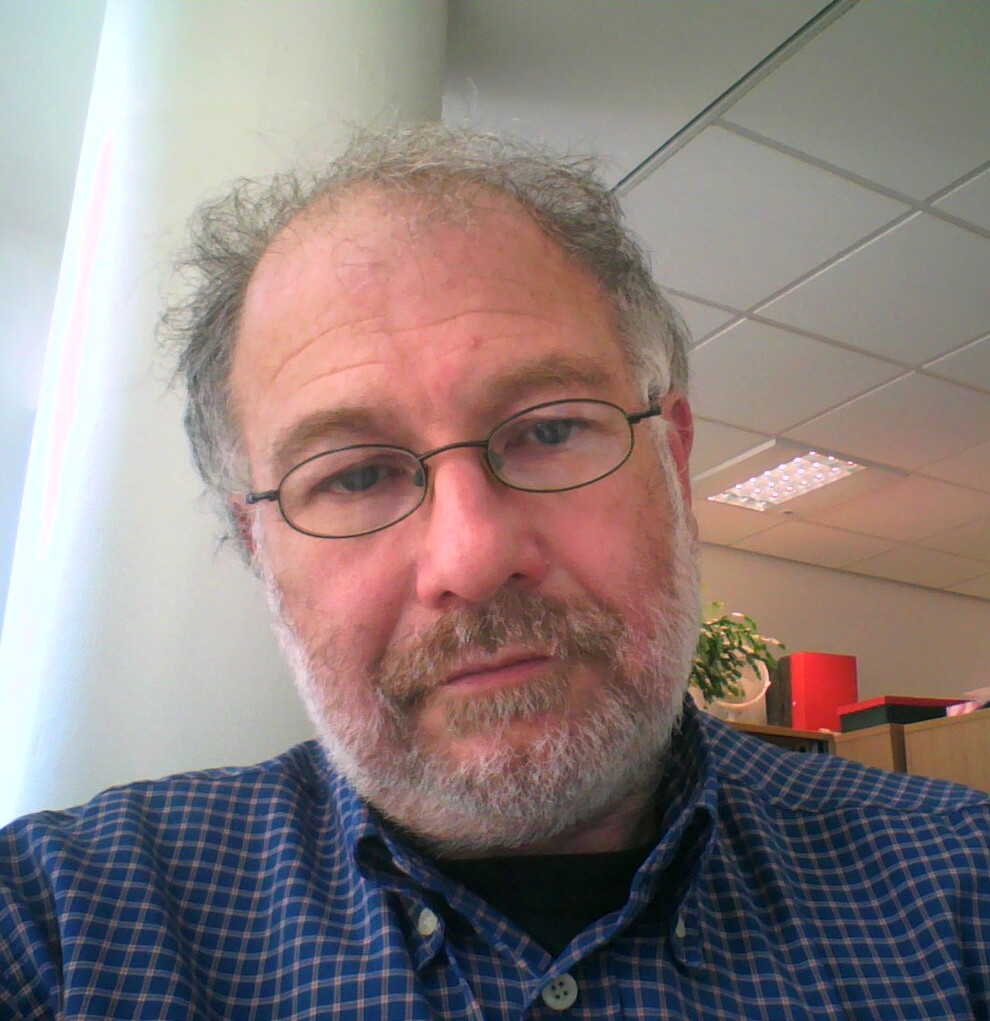
\includegraphics[width=1in,height=1.25in,clip,keepaspectratio]{Images/MB}}]{Michael Brockway}
has been a Senior Lecturer at Northumbria University for 17 years. His first degree is in pure and applied mathematics (1973-4), his Masters in mathematics (mathematical logic, category theory, 1975), and he has a PhD in computer science (formal methods for distributed embedded systems, 2010) from Northumbria University. Before that Michael worked in teaching and the computing industry.
\end{IEEEbiography}

\EOD

\end{document}

